\documentclass{GZUbachelorthesis}
\usepackage{listings}
\usepackage{subcaption}
\usepackage{xcolor}
\lstdefinestyle{mystyle}{
	backgroundcolor=\color{gray!10},
	commentstyle=\color{green!50!black},
	keywordstyle=\color{blue},
	numberstyle=\tiny\color{gray},
	stringstyle=\color{orange},
	basicstyle=\ttfamily\footnotesize,
	breakatwhitespace=false,
	breaklines=true,
	captionpos=b,
	keepspaces=true,
	numbers=left,
	numbersep=5pt,
	showspaces=false,
	showstringspaces=false,
	showtabs=false,
	tabsize=2,
	frame=single,
	rulecolor=\color{gray!30}
}
\makeatletter
\let\proof\relax
\let\endproof\relax
\makeatother
\usepackage{amsmath,amssymb,amsthm}
\usepackage{natbib}   
\usepackage{float} 
\usepackage{fancyhdr}
\usepackage{bm}
\usepackage{geometry}
\usepackage{graphicx}
\usepackage[colorlinks, 
linkcolor=black,
citecolor=black,
urlcolor=black   % 逗号已删除
]{hyperref}
\usepackage{enumitem} % 用于自定义列表标签 [label=(\alph*)]
% 实现首行缩进
\usepackage{indentfirst} % 让首行也缩进，符合中文习惯
%\setlength{\parindent}{0pt}     % 取消首行缩进（原设置，现注释掉）
%\setlength{\parskip}{1em}       % 增加段间距（可选，现注释掉）

\usepackage{newtxmath}   % 将数学字体设为 Times（含英文和数字）

% 减小公式上下方的间距
\setlength{\abovedisplayskip}{6pt}
\setlength{\belowdisplayskip}{6pt}
\setlength{\abovedisplayshortskip}{6pt}
\setlength{\belowdisplayshortskip}{6pt}
\usepackage{setspace} % 添加这个包
\renewcommand{\proofname}{证明}
\makeatletter
\renewenvironment{proof}[1][\proofname]{\par
	\normalfont
	\topsep6\p@\@plus6\p@\relax
	\trivlist
	\setlength{\itemindent}{2em}%
	\item[\hskip\labelsep{\songti #1：}]\ignorespaces
}{\hfill\ensuremath{\square}\endtrivlist\@endpefalse}
\makeatother
% 设置段落内部的行距为1.5倍
\setstretch{1.5}
% 在导言区（\begin{document}之前）添加以下宏定义
	\newcommand{\Oh}{\Omega}
	\newcommand{\Vh}{V_h}
	\newcommand{\Th}{\mathcal{T}_h}
	\newcommand{\norm}[1]{\left\| #1 \right\|}
	\newcommand{\abs}[1]{\left| #1 \right|}
	\titlepageset{
		title = {利用有限元方法数值求解热传导方程}, %论文标题,可用\\手动分行
		title* = {Numerical Solution of the Heat Conduction Equation Using the Finite Element Method}, %论文英文标题
		department = {数学与统计学院}, %学院
		major = {数学与应用数学}, %专业
		majorcode = {070101}, %专业代码
		class = {应数2201}, %班级
		studentID = {2200100100}, %学号
		author = {张雨}, %作者姓名
		author* = {Zhang Yu}, %作者英文姓名
		teacher = {刘鸿雁}, %指导老师
		date = {2026年6月5日}, %日期
	}
	\graphicspath{{figures/}} %定义所插入的图片均在figures文件夹内
	% 定义新的定理样式：正文字体、首行缩进
	\newtheoremstyle{chineseplain}% 样式名称
	{6pt}% 上方间距
	{6pt}% 下方间距
	{\normalfont}
  {2em} 
	{\bfseries}% 标题字体（粗体）
	{.}% 标题后标点
	{ }% 标题后与正文的间距
	{}% 标题规格（默认）
	
	% 将该样式应用于所有定理类环境
	\theoremstyle{chineseplain}
	% 定义定理环境
\newtheorem{theorem}{定理}[section]
\newtheorem{lemma}[theorem]{引理}
\newtheorem{corollary}[theorem]{推论}
\newtheorem{proposition}[theorem]{命题}
\newtheorem{definition}{定义}[section]
\newtheorem{example}{例}[section]
\newtheorem{remark}{注}[section]
\newtheorem{assumption}{假设}[section]
\begin{document}
\maketitle %生成封面页和诚信责任书

\begin{tocabstract} %生成目录和摘要
\begin{abstract}[热传导方程，有限元方法，稳定性，误差估计，数值实验] %中文摘要
热传导方程是描述介质内部热量随时间扩散传递规律的抛物型偏微分方程，广泛应用于工程传热、岩土勘探、智能控制、材料热处理等传统与新兴工程领域，是刻画多物理场综合作用、优化工程算法和揭示介质热动力学特性的重要数学工具。

本文以热传导方程的数值解法为核心研究内容，由理论到实践的研究思路，从一维非稳态热传导问题出发，并进一步将数值方法推广至二维情形。研究的基本思路如下：首先，基于分片线性有限元方法（P1）对空间变量进行离散，建立热传导方程的空间半离散格式，并对该半离散格式进行稳定性分析与误差估计；然后，在空间半离散的基础上，进一步在时间项采用二阶向后差分格式（BDF2）进行离散，构造全离散的BDF2-P1格式，并从理论上严格分析其稳定性与收敛性质；最后，借助编程工具实现一维和二维热传导问题的数值模拟，通过数值实验验证所提方法的有效性与实用性，为热传导方程的工程实际应用提供可靠的数值支撑。
\end{abstract}
\begin{enabstract}[Heat Conduction Equation, Finite Element Method, Stability, Error Estimate, Numerical Experiments] %英文摘要
The heat conduction equation is a parabolic partial differential equation that describes the law of heat diffusion and transfer within media over time. It is widely applied in traditional and emerging engineering fields including engineering heat transfer, geotechnical exploration, intelligent control, and material heat treatment. It is a crucial mathematical tool for characterizing the comprehensive effects of multi-physical fields, optimizing engineering algorithms and revealing the thermokinetic properties of media.
	
This thesis takes the numerical solution of heat conduction equations as its core research focus and adopts a theory-to-practice research framework. It first investigates one-dimensional unsteady heat conduction problems, and further extends the relevant research to two-dimensional cases. The fundamental research methodology is structured as follows: First, the spatial variables are discretized using the piecewise linear finite element method (P1) to establish a spatial semi-discrete scheme for the heat conduction equation, followed by a stability analysis and error estimation of this semi-discrete scheme. Subsequently, based on the spatial semi-discretization, the time term is discretized using the second-order backward difference formula (BDF2) to construct a fully discrete BDF2-P1 scheme, and its stability and convergence properties are rigorously analyzed in theory. Finally, numerical simulations of one-dimensional and two-dimensional heat conduction problems are implemented via programming tools. Numerical experiments validate the efficacy and practicability of the proposed method, providing reliable numerical support for engineering applications of the heat conduction equation.
\end{enabstract}
\end{tocabstract}
\section{绪论}
本章将叙述热传导方程的研究背景和意义，有限元方法数值求解热传导方程的优势，并综述有限元方法在数值求解热传导方程的国内外现状及应用，明确本文的主要内容和结构框架。
\subsection{研究背景与意义}
热传导方程是一种典型的线性抛物型偏微分方程，用于描述热量在介质中随时间的扩散过程，在工程传热分析、地热模拟、材料热处理等诸多领域具有较强的应用价值。值得大家注意的是，热传导方程的应用已经从传统的传热分析拓展到诸多新兴领域，其影响之广泛、形式之多样。例如，在工程控制领域，李滨等\cite{li2026improved}提出的改进人工势场与热传导混合算法，通过求解温度分布函数修正斥力势场，有效地解决了无人机路径规划中的目标不可达和局部最小值问题，即利用热传导方程的数学特性改进路径规划算法；在岩土工程领域，徐静茹等\cite{xu2025thermal}针对饱和冻土这一特殊地质介质，基于运动方程、本构方程与广义热传导方程，构建了多孔热弹性介质波动方程，系统分析了热效应作用下平面S1波的入射反射规律，揭示了热通量相位延迟时间、热传导系数、温度和接触参数对地震响应的影响机制；热传导方程则作为本构关系的核心组成部分，用于描述复杂环境下的多物理场综合作用现象，这里的“多物理”，通常指两个及以上不同物理过程（如力学变形、流体渗流、电磁感应等）在同一系统中同时发生并相互影响的复杂现象。

上述两个研究案例都从不同的角度展示了热传导方程的重要性，它既是解决工程算法缺陷的创新工具，又是揭示复杂介质物理机制的理论基础。然而在复杂几何构型、时变材料属性及复杂边界条件下，热传导方程的解析解往往难以获得甚至不存在，因此数值方法成为求解热传导方程的一个主要途径； 随着不断发展的工业技术，对热过程进行精确数值模拟的需求也日益剧增。

本文旨在探究利用有限元方法数值求解热传导方程的相关理论知识与数值验证，其研究意义主要体现在以下两个方面：理论意义是通过对一维热传导方程的空间半离散格式及全离散BDF2-P1格式的稳定性分析与误差估计，深化对偏微分方程数值解法的理论认识，尤其是对有限差分法与有限元方法相结合的高阶离散格式的数学性质有了更为清晰的把握；本文所建立的理论框架与分析方法，不仅适用于热传导方程，而且可以推广至一般抛物型方程，为其数值解法的设计、分析与优化提供具有一定普适性的理论工具与参考依据。实际意义是本文的研究成果是对工程热分析、材料科学、环境模拟等领域中热扩散过程的精确仿真；所推广的二维模型及FreeFem++实现，降低了热传导问题数值模拟的技术门槛。
\subsection{国内外研究现状}
%在众多数值方法中，有限差分法具有直观的数学推导和简便的实现方式的特点，始终是求解热传导方程最为经典的途径之一\cite{loskor2022numerical}。典型的差分格式包括Forward-Time Central-Space格式、Crank-Nicolson格式等\cite{mojumder2023efficient}。近年来，学者们愈发关注不同边界条件对差分格式稳定性与精度的影响，并发展了一系列适用于复杂边界的改进格式。例如，Maturi等人分析了铜材料瞬态热传导方程的有限差分逼近格式\cite{maturi2020finite}；Mojumder等人提出了一种高效的一维热方程有限差分法，并系统分析了其稳定性条件\cite{mojumder2023efficient}。然而，随着求解区域几何形态的复杂化及边界条件的多样化，有限差分法在灵活性上的局限日益凸显，难以适配复杂场景的求解需求\cite{lei2024review}。相比之下，基于变分原理与分片插值的有限元方法，在处理不规则区域和复杂边界方面展现出独特优势，成为弥补有限差分法不足的重要替代方案\cite{chen2010finite}。有限元法在处理复杂区域和非齐次边界条件方面具有明显优势，其基本思想是将连续的求解区域离散为一组有限个且按一定方式相互联结在一起的单元的组合体\cite{王晓峰2008轻型载重汽车正面碰撞控制结构分析与改进}。Dhawan等人采用三次B样条基函数对一维热方程进行了数值求解，展示了有限元法在格式构造上的灵活性\cite{dhawan2009numerical}。雷娜等人对有限元网格生成方法进行了系统综述，指出了有限元法在处理复杂几何区域时的核心优势与发展脉络\cite{lei2024review}。陈锡栋等人亦从工程应用视角梳理了有限元法的发展现状，强调了其在多物理场耦合问题中的关键地位\cite{chen2010finite}。此外，有限体积法作为介于有限差分与有限元之间的数值方法，也在热传导问题的求解中具有一定地位。Asish对扩散方程的有限体积解法进行了系统研究\cite{asish2016finite}；Saptaningtyas等人采用显式有限体积法对热方程进行了数值探索，进一步丰富了热传导问题的数值方法体系\cite{saptaningtyas2018finite}。近年来，国内外学者围绕热传导方程数值求解的空间离散策略、时间推进格式及全离散格式的稳定性与收敛性分析等方面，取得了丰硕成果。研究趋势已逐渐从单一方法的应用，转向更高精度、更强稳定性、更好适应复杂几何与多物理场耦合问题的多元化发展格局。Adomian提出的分解法更是为偏微分方程的解析与数值求解提供了新的视角\cite{adomian1994solution, adomian1998review}；Gorgus等人对比分析了热传导方程的不同数值求解方法，为方法选择提供了理论依据\cite{gorguis2008heat}。具体而言，有限元法求解热传导方程的研究正沿着三个方向深入推进：一是通过优化离散格式，提升对复杂热传导过程的模拟精度与稳定性，完善误差估计体系\cite{adomian1994solution}；二是结合自适应技术与多场耦合框架，突破传统方法的应用局限，拓展其在复杂几何与多物理场耦合问题中的适配能力\cite{lei2024review,chen2010finite}；三是借助并行计算与高效算法设计，提升大规模热传导问题的求解效率，满足工程中的高效仿真需求\cite{李荣华2010偏微分方程数值解法}。
在众多数值方法中，有限差分法、有限体积法与有限元方法是求解热传导方程的三类方法。有限差分法因直观的数学推导和简易的实现方式，始终是经典之选\cite{loskor2022numerical}；有限体积法介于有限差分法与有限元法之间，在保证物理量守恒性方面具有天然优势，在热传导问题的求解中也占据重要地位；有限元方法则基于变分原理与分片插值，在处理复杂几何区域和非齐次边界条件方面展现出独特优势\cite{chen2010finite}。

三种方法在历史发展上依次递进且各有侧重。有限差分法最早成熟，其核心在于利用差商逼近导数，格式构造简单，但受制于规则网格，难以适应复杂区域；典型的差分格式有时间向前差分、空间中心差分格式和Crank-Nicolson格式等\cite{mojumder2023efficient}。近年来，越来越多的学者愈发关注不同边界条件对差分格式稳定性与精度的影响，并发展了一系列适用于复杂边界的改进格式。例如，Nchupang等人将不可压缩的纳维–斯托克斯方程写成斜对称形式，并对边界条件施加弱限制，从而在角点上无需特殊处理即可实现有界性；在离散环境中，他们采用高阶有限差分法（SBP）模拟连续过程，并辅以弱边界条件，使用同时近似项（SAT）技术，随后通过SBP-SAT框架正式证明了稳定性\cite{Nchupang2025}；Mojumder等人提出了一种高效的一维热方程有限差分法，并分析了其稳定性条件\cite{mojumder2023efficient}。有限体积法随后在工程流体力学领域兴起，通过控制体积积分实现守恒性，兼顾了差分法的简洁与物理意义的清晰。例如，Asish对扩散方程的有限体积解法进行了系统研究\cite{asish2016finite}；Saptaningtyas等人采用显式有限体积法对热方程进行了数值探索，进一步丰富了热传导问题的数值方法体系\cite{saptaningtyas2018finite}。相比之下，有限元方法的发展较晚，其思想源于结构力学，后经数学理论完善形成独立分支，以变分原理和分片插值为根基，能够灵活处理不规则边界与材料非均匀性，成为弥补前两者局限的重要方案\cite{lei2024review,chen2010finite}。比如，准三维有限元方法因具有容易处理计算区域尺寸与土层厚度相差几个数量级的矛盾、对边界条件适用性强、计算效率高等特点，在多层地基复杂条件下的区域渗流计算中展现出独特优势\cite{mei2023quasi3D}。通过之前学者的研究，利用有限元方法求解热传导问题的研究已形成清晰的发展脉络，早期研究侧重于基本理论框架的建立与格式构造，如Dhawan等人采用三次B样条基函数对一维热方程进行数值求解，展示了有限元方法在基函数选取上的灵活性\cite{dhawan2009numerical}；随后，研究重点逐渐转向网格生成技术，雷娜等人系统综述了有限元网格的生成方法，指出其在处理复杂几何区域时的核心优势与发展脉络\cite{lei2024review}。进入二十一世纪，有限元方法在工程应用层面快速拓展，陈锡栋等人从工程视角梳理了其发展现状，强调了其在多物理场综合作用问题中的关键地位\cite{chen2010finite}。此外，Adomian提出的分解法为偏微分方程的数值求解提供了新的视角\cite{adomian1994solution, adomian1998review}；Gorgus等人对比分析了热传导方程的不同数值求解方法，为选择不同方法提供了理论依据\cite{gorguis2008heat}。

由此可见，有限元方法求解热传导问题的研究沿着三个方向深入推进：一是通过优化离散格式，提升对复杂热传导过程的模拟精度与稳定性，完善误差估计体系\cite{adomian1994solution}；二是结合自适应技术与多场综合作用框架，突破传统方法的应用局限，拓展其在复杂几何与多物理场问题中的适配能力\cite{lei2024review,chen2010finite}；三是借助并行计算与高效算法设计，提升大规模热传导问题的求解效率，满足工程中的高效仿真需求。总的来说，热传导方程数值求解的研究已从单一方法的应用，转向更高精度、更强稳定性、更好适应复杂几何与多物理场综合作用问题的多元化发展格局。
\subsection{本文主要内容}
%本文以带Dirichlet边界条件的热传导方程为研究对象，系统阐述其数学模型、弱形式推导、有限元离散格式构造以及相应的稳定性与误差分析，为后续数值实验奠定理论基础。首先，介绍带Dirichlet边界条件的热传导方程的数学模型，在模型的基础上，通过引入测试函数并利用格林公式，将原方程的强形式转化为积分意义下成立的弱形式。这一转化过程自然引出了Sobolev空间，能够有效降低对解的光滑性要求，使方程在更广泛的函数类中可解，为后续有限元分析提供了坚实的数学基础。随后，叙述了利用有限元方法数值求解热传导方程的基本思路，对变分形式离散化得到空间半离散格式，为进一步实现对时间变量的离散，引入二阶向后差分格式对时间导数进行逼近，从而得到全离散的BDF2-P1格式，这一格式将偏微分方程完全离散化为一系列线性代数系统，便于计算机求解。在此基础上，对所构造的半离散格式和全离散格式分别进行稳定性分析和误差估计。最后，通过选取具有精确解的一维、二维热传导方程数值算例，对前文的理论分析结果进行验证。同时，数值实验将考察不同网格尺寸和时间步长下数值解的收敛行为，验证理论分析所得的收敛阶；评估格式在实际应用中的有效性和可靠性。
本文以带齐次Dirichlet边界条件的热传导方程为研究对象，系统阐述其数学模型、弱形式推导、有限元离散格式构造以及相应的稳定性与误差估计，为后续数值实验奠定理论基础。

首先，介绍带齐次Dirichlet边界条件的热传导方程的数学模型，明确其在给定边界温度条件下的初边值问题描述；在此基础上，通过引入具有光滑性的测试函数，并利用格林公式对空间导数进行分部积分，将原方程（强形式）转化为在积分意义下成立的弱形式，这一转化过程自然引出了Sobolev空间，使得方程对解的光滑性要求降低，即方程可在更广泛的函数类中寻求解，从而为后续有限元分析的适定性提供了严谨的数学框架。

其次，叙述利用有限元方法数值求解热传导方程的基本思路；基于弱形式，通过构造有限维逼近子空间（如P1空间）对变分形式进行离散，得到关于时间的空间半离散格式，将原偏微分方程转化为常微分方程组；为进一步实现对时间变量的离散，引入二阶向后差分格式（BDF2）对时间导数项进行逼近，结合空间有限元离散，从而建立全离散的BDF2-P1格式，该格式将原偏微分方程完全离散化为一系列仅涉及代数方程组的线性系统，便于在计算机上高效求解。

最后，对所构造的半离散格式和全离散格式分别进行稳定性分析和误差估计，从理论上保证数值解在长时间积分下的有界性以及逼近解与真解之间的收敛性；通过选取具有精确解的一维和二维热传导方程数值算例，对前文的理论分析结果进行验证。同时，数值实验将考察不同网格尺寸和时间步长下数值解的收敛行为，验证理论分析所得的收敛阶，评估格式在实际应用中的有效性和可靠性。
\subsection{本文结构安排}
第一章阐述热传导方程和有限元方法的研究背景与意义，综述数值求解热传导方程的国内外相关研究现状和发展趋势，明确本文的主要内容和结构框架。

第二章介绍本文所需要的数学基础知识，包括Sobolev空间的基本概念与性质、有限元空间的构造、椭圆投影算子的定义及其性质、热传导方程的数学模型及其变分形式等，为后续的数值格式构造与分析奠定理论基础。

第三章介绍带齐次Dirichlet边界条件的热传导方程的有限元分析。首先建立其半离散有限元格式，并分析该格式的稳定性与收敛性；接着结合二阶向后差分格式（BDF2）对时间项进行离散，构造全离散BDF2-P1格式，并系统研究该格式的稳定性条件与误差估计。

第四章设计具有精确解的一维、二维及其非线性热传导方程模型问题，通过数值实验验证第三章中理论分析的有效性与可靠性。具体包括：观察不同网格尺寸和时间步长下数值解的收敛行为，验证理论收敛阶；通过对数值结果的可视化展示，直观呈现数值解对精确解的逼近效果。

第五章总结全文并展望未来可能的研究方向。
\newpage
\section{预备知识}
为后文进行有限元离散和数值分析的需要，本章给出相关的函数空间、椭圆投影算子以及变分形式，为建立热传导方程的有限元格式及其理论分析奠定理论基础。
\subsection{Sobolev空间和重要不等式}
设$\Omega \subset \mathbb{R}^d$（$d=1,2$）是一个具有Lipschitz连续边界$\partial\Omega$的有界连通区域，通过之前所学可知 \(L^p(\Omega)\) 表示 \(\Omega\) 上 \(p\) 次 Lebesgue 可积函数构成的等价类空间，其定义如下：
\[
L^p(\Omega) = \left\{ f: \Omega \to \mathbb{R} \text{ 可测}: \int_{\Omega} |f(x)|^p \, dx < \infty \right\},
\]
该空间配备的标准范数为：
\[
\|f\|_{L^p(\Omega)} = \left( \int_{\Omega} |f(x)|^p \, dx \right)^{1/p}, \quad 1 \leq p < \infty.
\]
特别地，$L^2(\Omega)$为$\Omega$上平方可积的函数空间，其内积与范数分别为 $(\cdot,\cdot)$ 和 $\|\cdot\|_{L^2(\Omega)}$，其具体形式为
\[
\left\{
\begin{aligned}
	(u,v)&=\displaystyle\int_\Omega u(x)v(x)\,\mathrm{d}x, \\
	\|u\|_{L^2(\Omega)} &= \displaystyle\left(\int_\Omega |u(x)|^2\,\mathrm{d}x\right)^{\frac{1}{2}}.
\end{aligned}
\right.
\]
Sobolev空间是为了适应本文对数值解光滑性要求较低的需求而引入的，对非负整数$m$，定义Sobolev空间：
\[
H^m(\Omega) = \left\{ v \in L^2(\Omega) : D^{\alpha} v \in L^2(\Omega) \text{ 对所有 } |\alpha| \le m \right\},
\]
其中$\alpha$为重指标，$H^m(\Omega)$上的范数（全范数）与半范数分别定义为
\[
\left\{
\begin{aligned}
	\| v \|_{m, \Omega} &= \left( \sum_{|\alpha| \leq m} \| D^\alpha v \|_{0, \Omega}^2 \right)^{1/2}, \\
	| v |_{m, \Omega}   &= \left( \sum_{|\alpha| = m} \| D^\alpha v \|_{0, \Omega}^2 \right)^{1/2}.
\end{aligned}
\right.
\]
特别地，$H^m_0(\Omega)$为$H^m(\Omega)$中在边界$\partial\Omega$迹为零的函数构成的子空间，即满足了齐次Dirichlet边界条件，成为热传导方程弱形式分析的恰当函数空间。

为了后文的理论分析，本节将列出几个重要不等式\cite{Wang2004,li2023shuxuewuli}。

（1）\textbf{Cauchy-Schwarz不等式 } \enspace
设 \(f, g \in L^2(\Omega)\)，则有
\begin{equation}
	\left| \int_{\Omega} f(x) g(x) \, dx \right| 
	\leq \left( \int_{\Omega} |f(x)|^2 \, dx \right)^{1/2} 
	\left( \int_{\Omega} |g(x)|^2 \, dx \right)^{1/2}.
	\label{eq:cauchy1}
\end{equation}
同样地，在内积形式下：
\begin{equation}
	\|f \cdot g\|_{L^1(\Omega)} \leq \|f\|_{L^2(\Omega)} \|g\|_{L^2(\Omega)}.
	\label{eq:cauchy2}
\end{equation}

（2） \textbf{Young 不等式 } \enspace
设 \(a, b \geq 0\)，\(p, q > 1\) 且 \(\frac{1}{p} + \frac{1}{q} = 1\)，则有
\begin{equation}
	ab \leq \frac{a^p}{p} + \frac{b^q}{q}.
	\label{eq:young1}
\end{equation}
对于任意 \(\varepsilon > 0\)，有带\(\varepsilon\)的形式：
\[
ab \leq \varepsilon a^2 + \frac{1}{4\varepsilon} b^2, \quad \forall a, b \in \mathbb{R}.
\]
更一般的情形为
\begin{equation}
	ab \leq \frac{\varepsilon^p}{p} a^p + \frac{1}{q \varepsilon^q} b^q, \quad \forall \varepsilon > 0.
	\label{eq:young3}
\end{equation}

（3） \textbf{Minkowski 不等式 } \enspace
对任意 \(f, g \in L^p(\Omega)\)，成立：
\begin{equation}
	\|f + g\|_{L^p(\Omega)} \leq \|f\|_{L^p(\Omega)} + \|g\|_{L^p(\Omega)}, \quad \forall f, g \in L^p(\Omega),\ 
	\label{eq:minkowski}
\end{equation}
对于 \(p = \infty\) 的情形，Minkowski不等式依然成立，此时范数定义为本质supremum。该不等式在有限元误差估计中具有广泛的应用，常用于将总误差分解为若干子项之和并进行逐项估计。

（4） \textbf{Poincaré 不等式 } \enspace
如果 \(\Omega\) 为连通且在一个方向上有界的区域，则对每个非负整数 \(m \in \mathbb{N}\)，存在 \(C_p=\text{const} > 0\)，使得
\begin{equation}
	\|v\|_{m,\Omega} \leq C_p |v|_{m,\Omega}, \quad \forall v \in H_0^m(\Omega).
	\label{eq:poincare1}
\end{equation}
由Poincaré不等式可得其等价形式：
\[
\|u\|_{H^1(\Omega)}^2 = \|u\|_{L^2(\Omega)}^2 + \|\nabla u\|_{L^2(\Omega)}^2 \leq (C_p^2 + 1) \|\nabla u\|_{L^2(\Omega)}^2.
\]
显然也有：
\[	
\|\nabla u\|_{L^2(\Omega)}^2 \leq \|u\|_{H^1(\Omega)}^2.
\]
因此，可以得到以下范数等价关系：
\begin{equation}
	\frac{1}{\sqrt{C_p^2 + 1}} \|u\|_{H^1(\Omega)} \leq \|\nabla u\|_{L^2(\Omega)} \leq \|u\|_{H^1(\Omega)}.
	\label{eq:poincare4}
\end{equation}
\subsection{有限元空间与椭圆投影算子}
为了利用有限元方法数值求解热传导方程，本文需要将无穷维空间替换为有限维离散子空间。这里考虑一维情形下,令$\Omega=(a,b)\subset \mathbb{R}$，对$\Omega$进行网格剖分，其剖分为
\[
\mathcal{T}_h: a = x_1 < x_2 < \cdots < x_{N+1} = b.
\]
记第$i$个单元 $e_i = [x_i, x_{i+1}]$，单元长度$h_i = x_{i+1}-x_i$，网格尺寸参数$h = \max\limits_{1 \le i \le N} h_i$。若所有$h_i$ 相等，则称网格为一致剖分，此时$h = (b-a)/N$。本文设$\mathcal{T}_h(\Omega)$是$\Omega$的一个尺寸为$h$的正则网格剖分，$V_h \subset H^1_0(\Omega)$是基于网格剖分$\mathcal{T}_h(\Omega)$的协调有限元空间\cite{xu2025finite}，其中$V_h$为
\begin{equation}
	V_h = \left\{v_h \in C^0(\overline{\Omega}) : \left. v_h \right|_{[x_{i-1},x_i]} \in \mathrm{P}1, \ i = 2, \ldots, N+1,\ v_h(a) = v_h(b) = 0 \right\} \subset H^1_0(\Omega).
	\label{eq:Vh}
\end{equation}
为了便于数值实现，这里取$V_h$的一组线性基底$\{\phi_i\}_{i=1}^{N+1}$，满足节点处的插值条件：
\begin{equation}
	\phi_i(x_j) = \delta_{ij}, \quad i, j = 1, \ldots, N+1,
	\label{eq:fem-basis-property}
\end{equation}
其中$\delta_{ij}$为Kronecker符号。

上式\eqref{eq:fem-basis-property}具有局部支集，即每个基函数$\phi_i$仅在节点$x_i$附近的两个相邻单元上取非零值，而在其余区域恒为零，这一性质保证了总体刚度矩阵和总体质量矩阵呈现稀疏结构，其具体形式为
\begin{equation}
	\phi_i(x) =
	\begin{cases}
		\displaystyle \frac{x - x_{i-1}}{h}, & x \in [x_{i-1}, x_i], \\[6pt]
		\displaystyle \frac{x_{i+1} - x}{h}, & x \in [x_i, x_{i+1}], \\
		0, & \text{其他},
	\end{cases}
	\qquad i=2, \dots, N-1.
	\label{eq:hat_function}
\end{equation}
对于边界节点，由于边界条件 $u(0)=u(1)=0$，通常可仅取内部节点对应的基函数构造解空间但仍可形式地写出
\[
\phi_1(x) =
\begin{cases}
	\displaystyle \frac{x_2-x}{h}, & x \in [x_1, x_2], \\
	0, & \text{其他},
\end{cases}
\qquad
\phi_{N+1}(x) =
\begin{cases}
	\displaystyle \frac{x-x_N}{h}, & x \in [x_N, x_{N+1}], \\
	0, & \text{其他}.
\end{cases}
\]
为了更直观地理解基函数的构造与性质，有限元空间中一组典型基函数的图像如图\ref{fig:basis-functions}所示。
\begin{figure}[H]
	\centering
	\includegraphics[width=0.5\linewidth]{jihanshu.png}
	\caption{线性插值基函数示意图}
	\label{fig:basis-functions}
\end{figure}
全局线性插值仅利用单一的一次多项式对求解域进行整体拟合，逼近精度较低，难以适配复杂求解问题；因此有限元方法引入分片线性插值思想，将求解域剖分为若干离散单元，在每个单元上分别构造线性插值形式，通过单元节点衔接形成整体有限元空间。本文采用分片线性插值基函数构造有限元空间，当需要进一步提升数值解的精度时，可自然推广至分片二次插值基函数，一个参考单元上的分片二次插值基函数的图像如图\ref{fig:basis-functions-two}所示。
\begin{figure}[H]
	\centering
	\includegraphics[width=0.5\linewidth]{jihanshu-two.png}
	\caption{二次插值基函数示意图}
	\label{fig:basis-functions-two}
\end{figure}
值得注意的是，上述构造的有限元空间$V_h$是$H^1_0(\Omega)$的一个有限维逼近子空间，其逼近性质依赖于网格尺寸$h$以及分片多项式的次数；对于本文采用的分片线性元，当$h \to 0$时，$V_h$ 中的函数可以逼近$H^1_0(\Omega)$中的任意函数，且具有二阶收敛精度（在$L^2$范数意义下）。

对于二维情形，可类似地构造有限元空间。设$\Omega \subset \mathbb{R}^2$ 为多边形区域，在与前文不产生歧义情况下，$\mathcal{T}_h$ 为 $\Omega$ 的一个拟一致三角形剖分（或四边形剖分），$h$ 为网格尺寸参数；则定义其分片线性有限元空间：
\begin{equation}
	W_h = \left\{ v_h \in C^0(\overline{\Omega}) : \left. v_h \right|_e \in \mathrm{P}1(e), \, \forall e \in \mathcal{T}_h, \, \left. v_h \right|_{\partial\Omega} = 0 \right\} \subset H_0^1(\Omega),
	\label{eq:Wh}
\end{equation}
其中$e$为剖分单元，$\mathrm{P}1(e)$ 为单元$e$上的线性多项式空间；同理可选取节点基函数进行数值实现。

下面给出二维情形的三角形剖分和四边形剖分，如图\ref{fig:poufen}所示。
\begin{figure}[H]
	\centering
	\begin{subfigure}[b]{0.4\linewidth}   % 宽度缩小为 0.4
		\centering
		\includegraphics[width=\textwidth]{triangle_mesh.png}
		\caption{三角形网格剖分}
		\label{fig:triangle}
	\end{subfigure}
	\hfill
	\begin{subfigure}[b]{0.4\linewidth}   % 宽度缩小为 0.4
		\centering
		\includegraphics[width=\textwidth]{quad_mesh.png}
		\caption{四边形网格剖分}
		\label{fig:quad}
	\end{subfigure}
	\caption{二维网格剖分图}
	\label{fig:poufen}
\end{figure}

为了便于后文对离散格式进行误差估计，本节引入椭圆投影算子的概念，其算子是连接无穷维解空间与有限元子空间的重要工具。
\begin{definition}[椭圆投影]
	设$V_h \subset H^1_0(\Omega)$为由分片线性有限元构成的有限维子空间。椭圆投影算子$ P_h: H^1_0(\Omega) \to V_h $定义如下：对任意$ u \in H^1_0(\Omega) $，$ P_h u \in V_h $满足
	\begin{equation}
		\label{eq:elliptic-projection}
		a(P_h u, v) = a(u, v), \quad \forall v \in V_h.
	\end{equation}
\end{definition}
上述定义给出了一个由椭圆双线性形式$a(\cdot,\cdot)$诱导的重要投影算子，其核心思想是：在有限维子空间 $V_h$ 中寻找一个逼近 $P_h u$，使得它与原函数$u$在双线性形式 $a(\cdot,\cdot)$ 意义下无法被$V_h$中的任何检验函数所区分。即$P_h u$是$u$在$V_h$中关于能量内积$a(\cdot,\cdot)$的最佳逼近。由式\eqref{eq:elliptic-projection} 直接可得，对任意 $v \in V_h$有
\begin{equation}
	\label{eq:Galerkin}
	a(P_h u-u, v)=0.
\end{equation}
特别地，关系式\eqref{eq:Galerkin}为Galerkin正交性条件，该性质说明有限元投影误差在能量内积意义下，与有限元空间 $V_h$ 相互正交。Galerkin正交性是有限元方法误差分析的核心理论基础，该性质可将求解误差分解为函数逼近误差与子空间正交误差两部分，进而借助插值逼近理论对投影误差进行定量估计，为模型的先验误差分析提供重要理论支撑。

\subsection{热传导方程模型}
在本文的模型问题中，考虑带齐次Dirichlet边界条件的非稳态热传导方程：
\begin{equation}
	\label{eq:heat-conduction-model}
	\left\{
	\begin{aligned}
		\frac{\partial u}{\partial t} - \alpha \Delta u &= f(\boldsymbol{x},t), && (\boldsymbol{x},t) \in \Omega \times (0,T], \\
		u(\boldsymbol{x},0) &= u_0(\boldsymbol{x}), && \boldsymbol{x} \in \Omega, \\
     	u(\boldsymbol{x},t) &= 0, && (\boldsymbol{x},t) \in \partial\Omega \times (0,T],
	\end{aligned}
	\right.
\end{equation}
其中$u=u(\boldsymbol{x},t)$是物体的温度，$\alpha>0$是物体的热扩散率。热扩散率是一个描述热量在介质中传递速率的重要物理量\cite{mojumder2023efficient}，反映了材料内部温度趋于均匀化的能力，且它表征了热量从高温区域向低温区域扩散的快慢程度，是衡量材料对温度变化响应速度的重要指标。在热传导理论中，热扩散率 $\alpha$ 的数学定义为：
\begin{equation}
	\label{eq:thermal-diffusivity}
	\alpha = \frac{\lambda}{\rho c},
\end{equation}
其中$\lambda$为热导率（单位：W/(m·K)），表示材料传导热量的能力；$\rho$为材料密度（单位：kg/m$^3$），表示单位体积内物质的质量；$c$为比热容（单位：J/(kg·K)），表示单位质量材料升高单位温度所需要的热量。

从量纲分析角度可得热扩散率的单位为m$^2$/s，这与质量扩散系数等传递系数的单位一致，体现了其“扩散”的本质属性。热扩散率的大小直接影响热传导方程的时间演化行为：$\alpha$ 值越大，热量扩散越快，温度分布趋于均匀所需时间越短；反之，$\alpha$ 值越小，热量传递越缓慢，温度梯度持续的时间越长。在工程应用中，热扩散率是选择材料的重要依据：
（1）高$\alpha$材料具备快速的导热与均温特性，适用于散热器、热交换器等需高效散热或均温的场景。马兴琛的研究利用光热辐射背检测技术对紫铜、铝等高导热金属材料的验证测试表明，准确获取高导热材料的热扩散率对于保障散热器件的性能设计至关重要\cite{Ma2013}；
（2）低$\alpha$材料导热速率低，所以广泛应用于建筑保温层、高温设备隔热层里等隔热保温领域。杨杰的研究指出，随着新型建筑保温材料的不断涌现，准确测量其热扩散率等参数是推广应用的先决条件，并实测了EPS板、泡沫玻璃等典型保温材料的热扩散率数据，为建筑节能设计提供了基础依据\cite{Yang2014}。


从数值计算角度来看，热扩散率$\alpha$直接影响热传导方程时间项离散格式的稳定性条件。对于显式时间项离散格式，为保证数值计算的稳定性，时间步长$\tau$与空间步长$h$需满足下面的不等式：
\[
\frac{\alpha \tau}{h^2} \leq C,
\]
其中$C$为与离散格式相关的常数。本文针对常系数情形（$\alpha$为常数）展开研究，该情形对应材料热物性不随温度显著变化，可为后续研究更复杂的变系数和非线性热传导问题提供理论基础。

接着将给出本文模型问题的弱形式，为了简化下文的理论分析，这里假设$\alpha=1$。对于热传导方程\eqref{eq:heat-conduction-model}，通过阅读相关书籍\cite{李荣华2010偏微分方程数值解法}，可知在等式两边同时乘以测试函数$v(x)$并在区域 $\Omega$ 上积分，从而得到其弱形式。其中测试函数 $v(x)$ 属于适当的函数空间 $V=H^1_0(\Omega)$。这里选择$H_0^1(\Omega)$作为函数空间主要基于以下考虑：第一，该空间自然地包含了齐次Dirichlet边界条件$u|_{\partial\Omega}=0$，使得边界条件被直接纳入空间定义中，在变分形式中无需额外处理；第二，在推导弱形式时，需要对扩散项进行分部积分，若取测试函数$v \in H_0^1(\Omega)$，则边界项 $v|_{\partial\Omega}=0$ 自动消失，从而得到简洁的弱形式。此外，在 $H_0^1(\Omega)$ 上成立Poincaré 不等式，这意味着$\|u\|_V = \|\nabla u\|_{L^2(\Omega)}$，这是该空间上的一个等价范数。

考虑问题\eqref{eq:heat-conduction-model}的第一式，引入测试函数 $v \in V$，在 $\Omega$ 上积分并应用格林公式，得到弱形式：
\[
\biggl( \frac{\partial u}{\partial t}, v \biggr) + (\nabla u, \nabla v) = (f, v), \quad \forall v \in V,
\]
其中$(\cdot,\cdot)$表示$L^2(\Omega)$内积，即
\[
(u,v) = \int_{\Omega} u(\boldsymbol{x}) v(\boldsymbol{x}) \, d\boldsymbol{x}, \quad 
(\nabla u, \nabla v) = \int_{\Omega} \nabla u \cdot \nabla v \, d\boldsymbol{x}.
\]
给定初值条件：
\[
u(\boldsymbol{x},0) = u_0(\boldsymbol{x}), \quad \boldsymbol{x} \in \Omega.
\]
为了书写方便，这里引入双线性形式和右端项线性泛函：
\begin{equation}
	a(u,v) = \int_{\Omega} \nabla u \cdot \nabla v \, d\boldsymbol{x}, \qquad
	(f,v) = \int_{\Omega} f(\boldsymbol{x},t) v(\boldsymbol{x}) \, d\boldsymbol{x}.
	\label{eq:bilinear_forms}
\end{equation}
在上述符号\eqref{eq:bilinear_forms}下，问题\eqref{eq:heat-conduction-model}的弱形式为
给定$f \in L^2(\Omega)$（更一般地$f \in L^2(0,T; L^2(\Omega))$），求 $u(t) \in V$，使得
\begin{equation}
	\label{eq:weak-form}
	\left\{
	\begin{aligned}
		\biggl( \frac{\partial u}{\partial t}, v \biggr) + a(u,v) &= (f, v), && \forall v \in V, \; \text{a.e. } t \in (0,T], \\[4pt]
		u(\boldsymbol{x},0) &= u_0(\boldsymbol{x}), && \boldsymbol{x} \in \Omega.
	\end{aligned}
	\right.
\end{equation}
有了方程\eqref{eq:heat-conduction-model}的弱形式，根据经典教材得到对于变分问题\eqref{eq:weak-form}的解存在且唯一\cite{evans2010partial}。接下来考察原问题\eqref{eq:heat-conduction-model}的解（强解）和变分问题\eqref{eq:weak-form}的解（弱解）的关系，并且在适当的函数空间下，若弱解具有足够的光滑性，则弱解就是强解\cite{evans2010partial}。一般地，在极限意义下，一列弱解的适当极限收敛到强解，从而建立了强解和弱解在理论上的统一。
\subsection{本章小结}
本章围绕研究所需的理论基础展开，讨论如何将热传导方程模型问题转化为变分问题，从而降低方程对解的光滑性要求。首先介绍了Sobolev空间及其子空间，定义了对应的范数与半范数，为描述解的正则性和弱形式的适定性提供了基本函数框架；然后构建了相关的函数空间、有限元空间及其投影算子等基础理论；最后给出带齐次Dirichlet边界条件的热传导方程模型问题，推导了模型的弱形式并说明强解与弱解的关系，为后续有限元离散格式的建立奠定了理论基础。接下来，将讨论本文模型问题的空间半离散格式和时空全离散格式。
\newpage
\section{空间半离散形式及全离散BDF2-P1形式}
本章以前文构建的热传导模型\eqref{eq:heat-conduction-model}为研究对象，完成模型的离散与理论分析。首先对空间变量进行有限元离散，构建其空间半离散格式；在此基础上进一步对时间变量离散，推导得到全离散BDF2-P1格式。同时，对这两类离散格式进行稳定性分析与误差估计，为后续数值方法的有效性、可靠性提供完备的理论依据。
vvvvvvvvvvvvvvvvvvvvvvvvvvvvvvvvvvvvvvvvv\subsection{有限元离散}
本节针对热传导模型的空间变量开展离散处理，采用分片线性有限元完成空间离散，构建对应的有限元离散模型。
\subsubsection{空间半离散形式}
基于基函数\eqref{eq:hat_function}，任意$u_h \in V_h$可表示为时变系数与空间基函数的线性组合：
\[
u_h(x,t) = \sum_{j=2}^{N} u_j(t) \phi_j(x),
\]
其中 $u_j(t) = u_h(x_j,t)$ 为节点 $x_j$ 处的时变系数，即温度函数在节点上的值。这种分离变量的表示形式将原无穷维问题转化为关于系数 $\{u_j(t)\}_{j=2}^{N}$ 的常微分方程组，从而为后续的时间离散奠定了基础。

对于固定的$t \in [0,T]$，求$u_h(x,t) \in V_h$，使得
\begin{equation}
	\label{eq:patial-semidiscretization}
	\left\{
	\begin{aligned}
		\left( \frac{\partial u_h}{\partial t}, v \right) +  a(u_h,v) &= (f, v), && \forall v \in V, \\
		u_h(x,0) &= u_{0,h}(x), && x \in \Omega,
	\end{aligned}
	\right.
\end{equation}
其中$u_{0,h}$是$u_0(x)$在$V_h$中的某种近似，式\eqref{eq:patial-semidiscretization}就是一维热传导方程的空间半离散格式。
\subsubsection{稳定性分析和误差估计}
为了分析空间半离散格式的收敛性，需要明确有限元空间对精确解的逼近能力。由有限元插值理论可知，对于满足正则性假设的网格剖分，有限元空间$V_h$具有如下标准的逼近性质\cite{Wang2004}：
\begin{equation}\label{eq:approx_property}
	\inf_{v \in V_h} \left( \|u - v\|_{L^2(\Omega)} + h \|\nabla(u - v)\|_{L^2(\Omega)} \right) \leq C h^{k+1} \|u\|_{H^{k+1}(\Omega)}, \quad \forall u\in H^{k+1}(\Omega) \cap H^1_0(\Omega),
\end{equation}
其中$k \geq1$为有限元空间$V_h$中所用分片多项式的次数。不等式\eqref{eq:approx_property}表明，对于足够光滑的函数$u$，空间$V_h$中总存在一个逼近元（例如插值或椭圆投影），使得$L^2$误差以$h^{k+1}$阶收敛，梯度误差以$h^{k}$阶收敛，这与有限元方法的最佳收敛阶理论相吻合。

对于空间半离散问题\eqref{eq:patial-semidiscretization}，取测试函数 $v = u_h \in V_h$，则可得
\begin{align}
	\left( \frac{\partial u_h}{\partial t}, u_h \right) + a(u_h, u_h) &= (f, u_h),\quad \forall u_h \in V_h.
	\label{eq:fe-weak-form} 
\end{align}
本节定义离散能量：
\begin{align}
	E_h(t) = \frac{1}{2} \, \| u_h(t) \|_{L^2(\Omega)}^2.
	\label{eq:eh}
\end{align}
则式\eqref{eq:fe-weak-form}可以改写为
\begin{align}
\frac{d E_h}{d t} = - \left\| \frac{\partial u_h}{\partial x} \right\|_{L^2(\Omega)}^2 + (\, f, \, u_h \,).
\label{eq:fe-weak-form-two}
\end{align}
这里需要利用Poincar\'{e}不等式\eqref{eq:poincare1}和Cauchy-Schwarz不等式\eqref{eq:cauchy2}，由于$V_h\subset H^1_0(\Omega) $且有限元解也满足Poincar\'{e} 不等式，则存在常数$C_{P}$使得：
\[
\| u_h \|_{L^2(\Omega)} \leq C_{P} \, \| \nabla u_h \|_{L^2(\Omega)}.
\]
因此式\eqref{eq:fe-weak-form-two}可写为
\begin{equation}\label{eq:ehu}
\frac{dE_h}{dt} \leq -\frac{1}{C_{P}^2} \, \| u_h \|_{L^2(\Omega)}^2 + \| f \|_{L^2(\Omega)} \, \| u_h \|_{L^2(\Omega)}.
\end{equation}
式\eqref{eq:eh}即$ \| u_h \|_{L^2(\Omega)}=\sqrt{2E_h}$，将其代入式\eqref{eq:ehu}可得：
\begin{align}
\frac{dE_h}{dt} \leq -\frac{2}{C_{P}^2} \, E_h + \sqrt{2} \, \| f \|_{L^2(\Omega)} \, \sqrt{E_h}.
\label{eq:fe-weak-form-three}
\end{align}
由此可得式\eqref{eq:fe-weak-form-three}是关于$E_h$的常微分不等式，进行估计可得
\begin{align}
\| u_h(t) \|_{L^2(\Omega)} \leq e^{\frac{-t}{C_{P}^2}} \, \| u_h(0) \|_{L^2(\Omega)} + \int_0^t e^{-\frac{t-s}{C_{P}^2}}  \, \| f(s) \|_{L^2(\Omega)} \, ds.
\end{align}
由此可得到半离散有限元解的稳定性结论，其具体表述如下：
\begin{theorem}[半离散有限元解的稳定性]
	设有限元空间 $V_h \subset H_0^1(\Omega)$ 满足有限元逼近条件，$u_h(t) \in V_h$ 为方程\eqref{eq:fe-weak-form}对应的半离散有限元解，则 $u_h(t)$ 满足如下 $L^2$ 范数稳定性估计：
	\begin{equation}
		\label{eq:stability-estimate}
		\| u_h(t) \|_{L^2(\Omega)} \leq e^{-\frac{t}{C_{P}^2}} \, \| u_h(0) \|_{L^2(\Omega)} + \int_0^t e^{-\frac{t-s}{C_{P}^2}} \, \| f(s) \|_{L^2(\Omega)} \, ds,
	\end{equation}
	其中 $C_P$ 为Poincaré常数，$u_h(0) \in V_h$ 为初始值的有限元投影，$f(s)$ 为方程源项。
\end{theorem}
该估计表明，有限元解$u_h$在$L^2$范数意义下连续依赖于初始数据$u_h(0)$和源项$f$，从而保证了数值格式的稳定性。

根据有限元空间$V_h$的逼近性质\eqref{eq:approx_property}和椭圆投影算子的定义及其性质，本节可得到半离散有限元解的误差估计结论，其具体表述如下：
\begin{theorem}[半离散有限元解的误差估计]
设$u(x,t)$和$u_h(x,t)$分别是原问题\eqref{eq:heat-conduction-model}和空间半离散问题\eqref{eq:patial-semidiscretization}的解，且真解$u$满足正则性假设$u, \, u_t \in L^2(0,T; H^{k+1}(\Omega))$，则存在与网格尺寸$h$ 无关的常数 $C > 0$，使得以下误差估计成立：
\begin{align}
	\begin{split}
		\label{eq:corrected_error}
		\| u_h(x,t) - u(x,t) \|_{L^2(\Omega)}
		\leq &\; \| u_{0,h} - u_0 \|_{L^2(\Omega)} \\
		& + C h^{k+1} \left( \| u_0 \|_{H^{k+1}(\Omega)} + \int_0^t \| u_t(s) \|_{H^{k+1}(\Omega)} \, \mathrm{d}s \right).
	\end{split}
	\end{align}
\end{theorem}
\begin{proof}
	根据椭圆投影算子\eqref{eq:elliptic-projection},且可将总误差$e(t)$分解为如下形式，即
\begin{equation}\label{eq:error_decomposition_one}
	\begin{aligned}
		e(t)&=u_h(t)-u(t) \\
		&=\big( u_h(t)-P_h u(t) \big)+\big( P_h u(t)-u(t) \big)=\theta(t)+\rho(t).
	\end{aligned}
\end{equation}
因此对$e(t)$的估计可转化为分别对$\theta(t)$和$\rho(t)$进行估计。

首先是$\rho(t)$的估计，由椭圆投影的逼近性质$\|u-P_h u\|_{H^1(\Omega)} \leq C h^k \|u\|_{H^{k+1}(\Omega)}$，即存在常数$C>0$使得
	\begin{equation}
		\|\rho(t)\|_{L^2(\Omega)} = \|P_h u(t)-u(t)\|_{L^2(\Omega)} \leq C h^{k+1} \|u(t)\|_{H^{k+1}(\Omega)}.
		\label{eq:rho-estimate-one}
	\end{equation}
	利用$u(t)=u_0+\int_0^t u_t(s)\,\mathrm{d}s$和Minkowski不等式\eqref{eq:minkowski}有
	\begin{equation}
		\|u(t)\|_{H^{k+1}(\Omega)} \leq \|u_0\|_{H^{k+1}(\Omega)} + \int_0^t \|u_t(s)\|_{H^{k+1}(\Omega)}\,\mathrm{d}s.
		\label{eq:minkowski_estimate}
	\end{equation}
	将式\eqref{eq:minkowski_estimate}代入式\eqref{eq:rho-estimate-one}即得
	\begin{equation}
		\|\rho(t)\|_{L^2(\Omega)} \leq C h^{k+1} \left( \|u_0\|_{H^{k+1}(\Omega)} + \int_0^t \|u_t(s)\|_{H^{k+1}(\Omega)}\,\mathrm{d}s \right). 
		\label{eq:rho-estimate}
	\end{equation}
	下面是$\theta(t)$的估计：由于$P_h$与时间无关，在$u_t$足够光滑的前提下，微分算子与投影算子可交换则有 $(P_h u)_t = P_h u_t$。对任意$q \in V_h$，
	\[
		\begin{aligned}
		(\theta_t, q)+(\nabla \theta, \nabla q) 
		&=(u_{h,t}, q)+(\nabla u_h, \nabla q)-\big( P_h u_t, q \big)-(\nabla P_h u, \nabla q) \\
		&=(f,q)-\big( P_h u_t,q \big)-(\nabla  u, \nabla q) \quad (\text{由空间半离散格式\eqref{eq:patial-semidiscretization}}) \\
		&=(f,q)-(\nabla  u, \nabla q)-\big( P_h u_t,q \big) \\
		&=(u_t,q)-\big( P_h u_t,q \big) \\
		&=(u_t-P_h u_t,q) \\
		&=-(\rho_t,q).
	\end{aligned}
	\]
	因此$\theta(t)$满足如下的误差方程：
	\begin{equation}
		(\theta_t, q)+(\nabla \theta, \nabla q)=-(\rho_t,q), \quad \forall q \in V_h. 
		\label{eq:theta-error-equation}
	\end{equation}
	取 $q=\theta(t) \in V_h$ 代入式\eqref{eq:theta-error-equation}，得
	\[
	(\theta_t, \theta) + \|\nabla \theta\|_{L^2(\Omega)}^2 = -(\rho_t, \theta).
	\]
	注意到$(\theta_t, \theta)=\frac{1}{2} \frac{d}{dt} \|\theta\|_{L^2(\Omega)}^2$，且 $\|\nabla \theta\|_{L^2(\Omega)}^2 \geq 0$，于是
	\begin{equation}
		\frac{1}{2} \frac{d}{dt} \|\theta\|_{L^2(\Omega)}^2 \leq -(\rho_t, \theta) \leq \|\rho_t\|_{L^2(\Omega)} \|\theta\|_{L^2(\Omega)}.
		\label{eq:energy-derivative}
	\end{equation}
	对式\eqref{eq:energy-derivative}应用Young不等式\eqref{eq:young1}，则
	\begin{equation}
		\frac{1}{2}\frac{d}{dt}\|\theta\|^2_{L^2(\Omega)} \leq \|\rho_t\|_{L^2(\Omega)}\|\theta\|_{L^2(\Omega)} \leq \frac{1}{2}\|\rho_t\|^2_{L^2(\Omega)}+\frac{1}{2}\|\theta\|^2_{L^2(\Omega)}.
		\label{eq:young-inequality}
	\end{equation}
	所以式\eqref{eq:young-inequality}可改写为
	\begin{equation}
		\frac{d}{dt}\|\theta\|_{L^2(\Omega)} \leq \|\rho_t\|_{L^2(\Omega)}.
		\label{eq:theta-differential}
	\end{equation}
	式\eqref{eq:theta-differential}两边从0到$t$积分可得，
	\begin{equation}
		\|\theta(t)\|_{L^2(\Omega)} \leq \int_0^t \|\rho_t\|_{L^2(\Omega)} \mathrm{d}s+\|\theta(0) \|_{L^2(\Omega)}. 
		\label{eq:theta-integral}
	\end{equation}
	对于初值，
	\[
	\begin{aligned}
		\|\theta(0)\|_{L^2(\Omega)}
		&= \|u_h(0) - u(x,0) + u(x,0) - P_h u(x,0)\|_{L^2(\Omega)} \\
		&\leq \|u_{0,h} - u_0\|_{L^2(\Omega)} + \|u_0 - P_h u_0\|_{L^2(\Omega)} \\
		&\leq \|u_{0,h} - u_0\|_{L^2(\Omega)} + C h^{k+1} \|u_0\|_{H^{k+1}(\Omega)}.
	\end{aligned}
	\]
	为便于引用，将初值估计写为
	\begin{equation}
		\|\theta(0)\|_{L^2(\Omega)} \leq \|u_{0,h} - u_0\|_{L^2(\Omega)} + C h^{k+1} \|u_0\|_{H^{k+1}(\Omega)}.
		\label{eq:theta-initial}
	\end{equation}
	对于 $\rho_t$，利用投影的逼近性质得
	\begin{equation}
		\|\rho_t(s)\|_{L^2(\Omega)} = \|u_t(s) - P_h u_t(s)\|_{L^2(\Omega)} \leq C h^{k+1} \|u_t(s)\|_{H^{k+1}(\Omega)}.
		\label{eq:rhot-estimate}
	\end{equation}
	将式\eqref{eq:theta-initial} 和式\eqref{eq:rhot-estimate} 代入式\eqref{eq:theta-integral}，得到
	\begin{equation}
		\|\theta(t)\|_{L^2(\Omega)} \leq \|u_{0,h}-u_0\|_{L^2(\Omega)}+C h^{k+1} \|u_0\|_{H^{k+1}(\Omega)} + C h^{k+1} \int_0^t \|u_t(s)\|_{H^{k+1}(\Omega)}\,\mathrm{d}s. 
		\label{eq:theta-final}
	\end{equation}
	最后，因为$e(t)$的分解式\eqref{eq:error_decomposition_one}，所以利用三角不等式及结合式\eqref{eq:rho-estimate}和式\eqref{eq:theta-final}可得半离散有限元解的误差估计，即
	\begin{equation}
		\begin{aligned}
			\|u_h(x,t)-u(x,t)\|_{L^2(\Omega)}
			&\leq \|\theta(t)\|_{L^2(\Omega)} + \|\rho(t)\|_{L^2(\Omega)} \\
			&\leq \|u_{0,h}-u_0\|_{L^2(\Omega)} + C h^{k+1} \left( \|u_0\|_{H^{k+1}(\Omega)} + \int_0^t \|u_t(s)\|_{H^{k+1}(\Omega)}\,\mathrm{d}s \right) \\
			&\quad +C h^{k+1} \left( \|u_0\|_{H^{k+1}(\Omega)}+\int_0^t \|u_t(s)\|_{H^{k+1}(\Omega)}\,\mathrm{d}s \right) \\
			&\leq \|u_{0,h}-u_0\|_{L^2(\Omega)} \\
			&\quad +C h^{k+1} \left( \|u_0\|_{H^{k+1}(\Omega)}+\int_0^t \|u_t(s)\|_{H^{k+1}(\Omega)}\,\mathrm{d}s \right),
		\end{aligned}
		\label{eq:final-error-estimate}
	\end{equation}
	其中常数$C$在不同行可能不同，但最终均可合并为一个与 $h$ 无关的常数。
\end{proof}
\subsection{时空全离散}
此时已获得方程\eqref{eq:heat-conduction-model}在空间上离散的半离散形式\eqref{eq:patial-semidiscretization}。为了进行数值实验，仍需对时间导数项进行离散，在众多时间离散方案中，本文基于对计算效率和数值精度的权衡，选择使用二阶向后差分格式（BDF2），该格式不仅具有二阶时间精度，在保证精度的同时，对热传导这类抛物型方程具有良好的数值稳定性，能够有效抑制数值振荡。
\subsubsection{全离散BDF-P1形式}
对时间导数项采用二阶向后差分格式离散，其在第$m$个时间层的近似形式为：
\begin{equation}\label{eq:BDF2_approx}
	\frac{\partial u}{\partial t} \bigg|_{t=t_m} \approx \frac{3u^m - 4u^{m-1} + u^{m-2}}{2\Delta t},
\end{equation}
其中$t_m=m\Delta t,\quad m = 0,1,\dots$。
记$u_h^m$为$u(x,t)$在$t=t_m$时$x$的函数在$V_h$中的近似，即$u_h^m \approx u_h(x,t_m)$，$f^m = f(x, t_m)$，$\Delta t=\tau$。

将时间导数项的近似式\eqref{eq:BDF2_approx}代入空间半离散格式\eqref{eq:patial-semidiscretization}，可得 $t_m$ ($m \geq 2$) 时刻的全离散格式：求 $u_h^m \in V_h$，使得
\begin{equation}\label{eq:full_discrete_BDF2}
	\left( \frac{3u_h^m - 4u_h^{m-1} + u_h^{m-2}}{2\tau}, \, v\right) + a(u_h^m, v) = (\, f^m, \, v\,), \quad \forall v \in V_h.
\end{equation}
相应的初值条件为
\[
u_h^0 = u_{0,h}(x), \quad x \in \Omega.
\]
需要注意的是，BDF2为二阶两步格式，后续进行数值实验时需已知两个初始值（$u_h^0$ 和 $u_h^1$）。由于上述初值条件仅给出了第一个初始值$u_h^0$，因此本文采用单步格式（如向后欧拉法）求解得到 $u_h^1$，作为格式所需的第二个初始值，以保证数值计算的顺利进行，其中向后欧拉格式为：
\begin{equation}\label{eq:bdf1-formula}
	\dfrac{\partial u}{\partial t}\biggr|_{t=t_m} \approx \dfrac{u^m - u^{m-1}}{\Delta t}.
\end{equation}

将全离散格式\eqref{eq:full_discrete_BDF2}化简为
\begin{equation}\label{eq:final_discrete}
	\bigl( 3u_h^m, v \bigr) + 2\tau \, a(u_h^m, v) = \bigl( 2\tau f^m + 4u_h^{m-1} - u_h^{m-2}, v \bigr), \quad \forall v \in V_h.
\end{equation}
在建立了问题\eqref{eq:heat-conduction-model}的全离散BDF-P1格式之后，本节遵循与空间半离散格式相类似的分析思路，旨在为该全离散格式建立相应的稳定性判据和误差估计结果，从而完善其数值分析理论框架。
\subsubsection{稳定性分析和误差估计}
本节定义离散时刻的能量范数：
\begin{equation}\label{eq:discrete_energy}
	E_h^m=\frac{1}{4} \| u_h^m \|_{L^2(\Omega)}^2 + \frac{1}{4} \| 2u_h^m - u_h^{m-1} \|_{L^2(\Omega)}^2 + \frac{\tau}{2} \| \nabla u_h^m \|_{L^2(\Omega)}^2.
\end{equation}
将式\eqref{eq:final_discrete}改写为
\begin{equation}
	\label{eq:final_discrete-two}
	2\left ( 3u_h^m - 4u_h^{m-1} + u_h^{m-2},\; v \right) + 4\tau \, a(u_h^m, v) = 4\tau \left(  f^m,\; v \right), \quad \forall v \in V_h.
\end{equation}
\begin{theorem}[全离散BDF2-P1格式的稳定性]\label{thm:quanwend}
	设 $u_h^m$ 是式\eqref{eq:final_discrete}的解，源项 $f \in L^\infty(0,T; L^2(\Omega))$。则存在与 $\tau$，$h$ 无关的常数 $C > 0$，使得对任意 $m \geq2$，以下稳定性估计成立：
	\begin{equation}\label{eq:BDF2_stability_estimate}
		\| u_h^M \| + \tau \sum_{m=2}^M \| \nabla u_h^m \| 
		\leq C \left( \| u_h^0 \| + \| u_h^1 \|+ \tau \sum_{m=2}^M \| f^m \| \right),
	\end{equation}
	其中 $\| \cdot \|$ 表示 $L^2(\Omega)$ 范数，以下同是。特别地，当 $f \equiv 0$ 时，有$E_h^m \leq E_h^{m-1}$，表明离散能量随时间非增。
\end{theorem}
\begin{proof}
	在式子\eqref{eq:final_discrete-two}中，取测试函数 $v = u_h^m$，并利用BDF2的经典恒等式：
%	\begin{equation}\label{eq:BDF2_identity}
%		\begin{aligned}
%			2(3u_h^m &- 4u_h^{m-1} + u_h^{m-2}, u_h^m) = \\
%			&\| u_h^m \|^2 + \| 2u_h^m - u_h^{m-1} \|^2 - \| u_h^{m-1} \|^2 - \| 2u_h^{m-1} - u_h^{m-2} \|^2 + \| u_h^m - 2u_h^{m-1} + u_h^{m-2} \|^2,
%		\end{aligned}
%	\end{equation}
\begin{equation}
	\label{eq:BDF2_identity}
	\begin{aligned}
		& 2(3u_h^m - 4u_h^{m-1} + u_h^{m-2}, u_h^m) \\
		&= \| u_h^m \|^2 + \| 2u_h^m - u_h^{m-1} \|^2 - \| u_h^{m-1} \|^2 \\
		&\quad - \| 2u_h^{m-1} - u_h^{m-2} \|^2 + \| u_h^m - 2u_h^{m-1} + u_h^{m-2} \|^2.
	\end{aligned}
\end{equation}
	接着将恒等式\eqref{eq:BDF2_identity}代入式\eqref{eq:final_discrete-two}，整理可得：
	\begin{equation}\label{eq:energy_step}
		\begin{aligned}
			&\frac{1}{4\tau} \big( \| u_h^m \|^2 + \| 2u_h^m - u_h^{m-1} \|^2 - \| u_h^{m-1} \|^2 - \| 2u_h^{m-1} - u_h^{m-2} \|^2 \big) + \| \nabla u_h^m \|^2 \\
			&+ \frac{1}{4\tau} \| u_h^m - 2u_h^{m-1} + u_h^{m-2} \|^2 = (f^m, u_h^m).
		\end{aligned}
	\end{equation}
	利用Cauchy-Schwarz不等式\eqref{eq:cauchy2}和Young不等式\eqref{eq:young3}（取 $\varepsilon = 1$）估计右端项：
	\begin{equation}\label{eq:source_estimate}
		(f^m, u_h^m) \leq \| f^m \|\| u_h^m \| \leq  \frac{1}{2} \| f^m \|^2 + \frac{1}{2} \| u_h^m \|^2.
	\end{equation}
	将式\eqref{eq:source_estimate}代入式\eqref{eq:energy_step}，并忽略非负项 $\frac{1}{4\tau} \| u_h^m - 2u_h^{m-1} + u_h^{m-2} \|^2 \geq 0$，得到不等式：
%	\begin{equation}\label{eq:energy_ineq}
%		\frac{1}{4\tau} \big( \| u_h^m \|^2 + \| 2u_h^m - u_h^{m-1} \|^2 \big) + \| \nabla u_h^m \|^2 \leq \frac{1}{4\tau} \big( \| u_h^{m-1} \|^2 + \| 2u_h^{m-1} - u_h^{m-2} \|^2 \big) + \frac{1}{2} \| f^m \|^2 + \frac{1}{2} \| u_h^m \|^2.
%	\end{equation}
\begin{equation}
	\label{eq:energy_ineq}
	\begin{aligned}
		\frac{1}{4\tau} \big( \| u_h^m \|^2 + \| 2u_h^m - u_h^{m-1} \|^2 \big) + \| \nabla u_h^m \|^2 
		\leq &\; \frac{1}{4\tau} \big( \| u_h^{m-1} \|^2 + \| 2u_h^{m-1} - u_h^{m-2} \|^2 \big) \\
		& + \frac{1}{2} \| f^m \|^2 + \frac{1}{2} \| u_h^m \|^2.
	\end{aligned}
\end{equation}
	这里注意到 $\| u_h^m \|^2 \leq 4 E_h^m$，代入式\eqref{eq:energy_ineq}并结合\eqref{eq:discrete_energy}得：
\begin{equation}\label{eq:wen}
		\frac{1}{\tau} (E_h^m - E_h^{m-1}) +\left(1-\frac{\tau}{2}\right) \| \nabla u_h^m \|^2 \leq \frac{1}{2} \| f^m \|^2 + 2E_h^m.
\end{equation}
	式\eqref{eq:wen}两边乘以 $\tau$ 并移项,当时间步长 $\tau$ 满足 $0 < \tau \leq \frac{1}{4}$ 时，有 $1 - 2\tau \geq \frac{1}{2}$，则得：
	\begin{equation}\label{eq:final_recursion}
		E_h^m \leq 2 E_h^{m-1} + \tau \| f^m \|^2.
	\end{equation}
	对 $m = 2, 3, \dots, M$ 递归应用，可得：
	\begin{equation}\label{eq:diguishi}
	E_h^M \leq C \left( E_h^1 + \tau \sum_{m=2}^M \| f^m \|^2 \right),
	\end{equation}
	其中常数 $C=e^{2T}$，$T = M\tau$。进一步，由 $E_h^m$ 的定义及向量三角不等式
\begin{equation}
	\label{eq:inequalities}
	E_h^1 \leq C( \| u_h^0 \|^2 + \| u_h^1 \|^2 ),\quad 
	\| u_h^M \|^2 \leq 4E_h^M,\quad 
	\tau \| \nabla u_h^m \|^2 \leq 2E_h^m.
\end{equation}
	结合这些关系\eqref{eq:inequalities}，最终得到稳定性估计\eqref{eq:BDF2_stability_estimate}。
\end{proof}
\endproof
\begin{theorem}[全离散BDF2-P1格式的误差估计]\label{thm:quanwuc}
设$u(x,t_m)$和$u_h^m$分别是式\eqref{eq:heat-conduction-model}在$t=m\tau$和式\eqref{eq:final_discrete}的解，则满足如下误差估计（以下的$\|\cdot\|$都是$L^2$范数）：
\begin{equation}\label{eq:error-estimate}
	\max_{2 \leq m \leq M} \|u(t_m) - u_h^m\| \leq C (\tau^2 + h^{k+1}) \|u\|_{C^3([0,T];H^{k+1})},
\end{equation}
其中常数$C > 0$依赖于终时 $T$，但与 $\tau, h$ 无关。
\end{theorem}
\begin{proof}
定义椭圆投影误差和离散误差分别为：
\[
	\left\{
\begin{aligned}
	\eta(t) &= u(t) - P_h u(t), & t \in [0,T], \\
	e_h^m &= u_h^m - P_h u(t_m), & m = 0,1,\dots,M.
\end{aligned}
\right.
\]
则总误差可分解为：
\begin{equation}\label{eq:error-decomposition}
	u(t_m) - u_h^m = \eta(t_m) - e_h^m.
\end{equation}
在 $t = t_m$ 处，原连续方程\eqref{eq:heat-conduction-model}可写为：
\begin{equation}\label{eq:continuous-weak}	
	(u_t(t_m), v) + a(u(t_m),  v) = (f^m, v), \quad \forall v \in V_h.
\end{equation}
又因为$u(t_m)=P_h u(t_m)+\eta(t_m)$且由椭圆投影\eqref{eq:elliptic-projection}得$a(\eta(t_m),v)=0$则代入式子\eqref{eq:continuous-weak}：
\begin{equation}\label{eq:projection-weak}
	(\partial_{t} P_h u(t_m),v)+a(P_h u(t_m),v)=(f^m, v)-(\partial_{t} \eta(t_m),v), \quad \forall v \in V_h.
\end{equation}
对 $\partial_{t} P_h u(t_m)$进行二阶向后差分格式离散，定义：
\[
\partial_{t} P_h u(t_m)=\frac{3P_h u(t_m) - 4P_h u(t_{m-1}) + P_h u(t_{m-2})}{2\tau}+r^m.
\]
则误差方程为：
\begin{equation}\label{eq:error-equation}
	2\bigl( 3e_h^m - 4e_h^{m-1} + e_h^{m-2},\; v \bigr) + 4\tau a( e_h^m,  v) = 4\tau (R^m, v), \quad \forall v \in V_h,
\end{equation}
其中剩余项$R^m$为：
\begin{equation}\label{eq:R-def}
	R^m=\partial_{t} \eta(t_m)+ r^m.
\end{equation}

因为二阶向后差分格式具有二阶收敛，所以$\|r^m\| \leq C_1 \tau^2 \|u\|_{C^3([0,T];H^{k+1})}$，其中$C_1$是与时间导数有关的常数。又椭圆投影逼近满足
\begin{equation}
	\|\partial_{t} \eta(t_m)\| \leq C_2 h^{k+1} \|\partial_t u\|_{H^{k+1}(\Omega)},
\end{equation}
其中$h$为空间网格尺寸，$k$为有限元次数，$C_2$为与空间导数有关的常数。利用三角不等式使得$\|R^m\|$满足式\eqref{eq:rm}，其估计如下：
\begin{equation}\label{eq:rm}
	\|R^m\| \leq \|\partial_t \eta(t_m)\| + \|r^m\| \leq C_2 h^{k+1} \|\partial_t u\|_{H^{k+1}} + C_1 \tau^2 \|u\|_{C^3([0,T];H^{k+1})}.
\end{equation}
因此，整体截断误差具有空间$k+1$阶和时间二阶收敛性：
\begin{equation}
	\|R^m\| \leq C (h^{k+1} + \tau^2)\|u\|_{C^3([0,T];H^{k+1})},
\end{equation}
其中C为常数。

误差方程\eqref{eq:error-equation}与BDF2形式完全相同，仅右端项为$4\tau R^m$。因此，可直接应用全离散BDF-P1格式的稳定结论\eqref{thm:quanwend}估计于 $\{e_h^m\}$，得到：
\begin{equation}\label{eq:e-stability}
	\|e_h^M\|^2+ \tau \sum_{m=2}^M \|\nabla e_h^m\|^2 \leq C \left( \|e_h^0\|^2 + \|e_h^1\|^2 + \tau \sum_{m=2}^M \|R^m\|^2 \right).
\end{equation}

接着估计$\|e_h^0\|$和$\|e_h^1\|$，由于$e_h^0=u_h^0-P_h u(0),e_h^1=u_h^1-P_h u(\tau)$，取$u_h^0 = P_h u(0)$，则$\|e_h^0\| = 0$，对于$e_h^1$，本文采取向后欧拉法，即
\begin{equation}\label{eq:begin-error}
		\|e_h^1\| \leq C (h^{k+1} + \tau^2)\|u\|_{C^3([0,T];H^{k+1})}.
\end{equation}
将上述估计代入稳定性不等式\eqref{eq:e-stability}，并结合$\|R^m\| \leq C (h^{k+1} + \tau^2)\|u\|_{C^3([0,T];H^{k+1})}$，可得
\begin{equation}
	\|e_h^M\|^2 + \tau \sum_{m=2}^M \|\nabla e_h^m\|^2 \leq C (h^{k+1} + \tau^2)^2 \|u\|_{C^3([0,T];H^{k+1})}^2.
\end{equation}
对上式两边取平方根，并利用不等式$\sqrt{a+b} \leq \sqrt{a} + \sqrt{b} \leq \sqrt{2}\sqrt{a+b}$，有
\begin{equation}\label{eq:e-bound}
	\|e_h^M\| + \left(\tau \sum_{m=2}^M \|\nabla e_h^m\|^2\right)^{\frac{1}{2}} \leq C (h^{k+1} + \tau^2) \|u\|_{C^3([0,T];H^{k+1})}.
\end{equation}

接下来，由误差分解\eqref{eq:error-decomposition}和三角不等式，有
\begin{equation}\label{eq:triangle-l2}
	\|u(t_m) - u_h^m\| \leq \|\eta(t_m)\| + \|e_h^m\|.
\end{equation}
由椭圆投影算子的逼近性质，可得
\begin{equation}\label{eq:eta-bound}
	\|\eta(t_m)\| \leq C h^{k+1} \|u(t_m)\|_{H^{k+1}(\Omega)} \leq C h^{k+1} \|u\|_{C^3([0,T];H^{k+1})}.
\end{equation}
结合$\|e_h^m\|$的估计式\eqref{eq:e-bound}，并取$2 \leq m \leq M$上的最大值，即可得到全离散BDF2-P1格式的误差估计\eqref{eq:error-estimate}。
\end{proof}
%\subsection{方法向二维热传导方程的推广}
%\subsubsection{二维热传导方程模型}
%考虑二维区域 $\Omega \subset R^2$ 上的热传导方程：
%\begin{equation}
%	\begin{cases}
%		\dfrac{\partial u}{\partial t} - \alpha \Delta u = f(\boldsymbol{x}, t), & \boldsymbol{x} \in \Omega,\; t \in (0, T] \\
%		u(\boldsymbol{x}, 0) = u_0(\boldsymbol{x}), & \boldsymbol{x}\in \Omega \\
%		u(\boldsymbol{x}, t) = g(\boldsymbol{x}, t), & \boldsymbol{x} \in \partial\Omega,\; t \in (0, T]
%	\end{cases}
%	\label{eq:2d-heat-system}
%\end{equation}
%其中 $\alpha>0$ 为热扩散系数，$\Delta=\frac{\partial^2}{\partial x^2} + \frac{\partial^2}{\partial y^2}$ 为 Laplace 算子。
%\subsubsection{二维热传导方程半离散和全离散格式}
%对空间离散采用线性有限元，定义 Sobolev 空间 $V = H^1_0(\Omega)$。将方程两端乘以测试函数 $v \in V$ 并在 $\Omega$ 上积分,利用分部积分公式得到其有限元形式：
%\begin{equation}
%	\left( \frac{\partial u_h}{\partial t}, v \right) + \alpha (\nabla u_h, \nabla v) = (f, v), \quad \forall v \in W_h \label{eq:semidiscrete-weak}
%\end{equation}
%其中$(\cdot, \cdot)$表示$L^2(\Omega)$内积，$W_h \subset V$ 为有限元空间。
%
%接着对时间离散采用 BDF2 格式，记$u_h^n$ 为 $t_n = n\tau$时刻的数值解，则全离散格式为：
%\begin{equation}
%	\frac{1}{\tau} \left( \frac{3}{2} u_h^{n} - 2 u_h^{n-1} + \frac{1}{2} u_h^{n-2}, v \right) 
%	+ \alpha (\nabla u_h^{n}, \nabla v) = (f^{n}, v), \quad \forall v \in V_h \label{eq:bdf2-scheme}
%\end{equation}
\subsection{二维情形}
前文已详细叙述了热传导方程\eqref{eq:heat-conduction-model}的全离散BDF2-P1格式，本节将相同的数值框架推广至二维情形，考虑区域$\Omega \subset \mathbb{R}^2$下的热传导方程：
\begin{equation}
	\left\{
	\begin{aligned}
		\dfrac{\partial u}{\partial t} - \alpha \Delta u &= f(x,y,t), && (x,y) \in \Omega,\; t \in (0, T], \\
		u(x,y,0) &= u_0(x,y), && (x,y)\in \Omega, \\
		u(x,y,t) &= g(x,y,t), && (x,y) \in \partial\Omega,\; t \in (0, T],
	\end{aligned}
	\right.
	\label{eq:2d-heat-system}
\end{equation}
其中$\alpha>0$为热扩散系数，$ g(x,y,t)=0$，$\Delta=\frac{\partial^2}{\partial x^2} + \frac{\partial^2}{\partial y^2}$ 为Laplace算子。

观察方程\eqref{eq:2d-heat-system}与一维热传导方程\eqref{eq:heat-conduction-model}，可见在形式上并未有太大区别，但是二维模型在物理机理与数学表达上有着本质的区别。第一，一维问题仅描述沿单一空间方向的热量传递，未知函数为$u(x,t)$，扩散项仅包含$x$方向二阶偏导数；第二，二维模型描述平面区域内的温度场演化，未知函数扩展为$u(x,y,t)$，Laplace 算子包含$x$和$y$两个方向的二阶偏导数，热量在平面内沿所有方向同时扩散；第三，在边界形式上，一维问题边界仅为两个孤立点，二维问题边界为闭合平面曲线，边界条件的施加与处理更加复杂。

对空间离散仍采用分片线性有限元，定义Sobolev空间$V = H^1_0(\Omega)$。将方程两端乘以测试函数 $v(x,y) \in V$ 并在 $\Omega$ 上积分，利用分部积分公式得到其有限元半离散形式：
\begin{equation}
	\left( \frac{\partial u_h}{\partial t}, v \right) + \alpha (\nabla u_h, \nabla v) = (f, v), \quad \forall v \in W_h, \label{eq:semidiscrete-weak}
\end{equation}
其中$(\cdot, \cdot)$表示$L^2(\Omega)$内积，$W_h \subset V$ 为有限元空间，$W_h$的定义可见\eqref{eq:Wh}。

通过观察可知，一维与二维情形的空间半离散格式在数学形式上虽然保持一致，但是积分空间与微分算子有着明显差异。第一，一维格式的内积为区间上的定积分，梯度仅包含单方向偏导数；第二，二维格式的内积为平面区域上的二重积分，梯度为二维向量形式，离散后得到的质量矩阵与刚度矩阵均由二维网格积分组装而成，矩阵维度和计算量远大于一维格式。

对于有限元空间构造中选取的基函数，一维和二维情形也有着区别，一维线性元在每个单元上使用线性函数，整体基函数为“帽子函数”，形状简单，节点只与左右相邻单元关联；二维线性元（如三角形单元）的基函数在每个单元上为线性函数$\phi_i=a+bx+cy$，其支撑集为围绕节点$i$的所有单元构成的星形区域，节点自由度数量与网格节点数一致，但每个节点关联的单元数远多于一维，导致组装后的刚度矩阵带宽显著增大。尽管基函数的具体形式与支撑区域不同，但是它的核心作用是一样的。

接着对时间离散采用二阶向后差分格式\eqref{eq:BDF2_approx}，记$u_h^n$为$t_n = n\tau$时刻的数值解，则问题\eqref{eq:2d-heat-system}的全离散格式为：
\begin{equation}
	\frac{1}{\tau} \left( \frac{3}{2} u_h^{n} - 2 u_h^{n-1} + \frac{1}{2} u_h^{n-2}, v \right) 
	+ \alpha (\nabla u_h^{n}, \nabla v) = (f^{n}, v), \quad \forall v \in V_h.\label{eq:bdf2-scheme}
\end{equation}
全离散离散格式在一维与二维问题中形式完全相同，BDF2的二阶精度与稳定性可直接推广至二维情形。二者的核心区别体现在数值实现层面：一维全离散格式仅需处理一维网格与单元积分，二维格式则需要在三角形、四边形等二维单元上执行数值积分，完成单元矩阵组装与线性方程组求解。

\subsection{本章小结}
%本章针对一维热传导问题，构建了有限元空间半离散格式与全离散BDF2-P1格式，并系统分析了其数值稳定性与收敛性。首先，基于有限元空间，利用节点基函数将原问题转化为关于节点系数的常微分方程组，建立空间半离散格式；借助有限元插值理论，证明了半离散解在$L^2$范数下对初始数据与源项的连续依赖性。其次，通过引入椭圆投影算子，将误差分解为投影误差与离散误差，导出最优阶误差估计，收敛阶达$O(h^{k+1})$。接着，采用二阶向后差分格式离散时间导数，构造全离散BDF2-P1格式，证明在时间步长$\tau$满足特定条件时格式的稳定性，体现离散能量的非增性。进一步，通过误差分解与稳定性分析，获得全离散格式在$L^2$范数下的最优阶误差估计。最后，将一维情形的离散格式的构造方法推广至二维，阐述一维与二维情形的共同点和区别。综上，理论严格证明了该格式对一维热传导问题稳定且收敛，时间方向二阶精度，空间方向$L^2$范数下$k+1$阶最优收敛性，为数值实验提供了理论依据。
本章针对带齐次Dirichlet边界条件的一维热传导问题，构建了空间半离散格式与全离散BDF2-P1格式，并对两种格式的数值稳定性与收敛性进行了完整的理论分析。首先，建立空间半离散格式并证明其解的连续依赖性，通过椭圆投影算子导出最优阶误差估计；然后，构造其时空全离散格式并证明其稳定性，获得$L^2$范数下最优阶误差估计；最后，将一维情形下离散格式的构造思路与分析方法推广至二维热传导问题，详细阐述了一维与二维情形的共同点与核心区别，为后续二维问题的深入研究奠定基础。此外，为验证本文数值方法对非线性模型的适配性与有效性，第四章将结合具体的数值算例进行验证。
\newpage
\section{数值实验}
理论分析与数值验证相辅相成。前文已从理论上详细分析了空间半离散和时空全离散格式的稳定性与收敛性，本章将通过构造合适的数值算例，对该理论分析的正确性与有效性进行验证，从而为算法的实际应用提供依据。
\subsection{数值实例}
\textbf{例1.} 设定解问题：
\begin{equation}
	\begin{cases}
		u_t -\alpha u_{xx} = G \sin\left(\pi x\right), & 0 < x < 1,\; 0 < t <1, \\
		u(0,t) = 0, \quad u(1,t) = 0, & 0 \leq t < 1, \\
		u(x,0) = 0, & 0 \leq x \leq 1,
	\end{cases}
	\label{eq:test-problem}
\end{equation}
其中$\alpha = 1$， $G = 2$。
用分离变量法求解定解问题\eqref{eq:test-problem}的解析解为：
\begin{equation}
	u(x,t) = \frac{2}{\pi^2} \left(1 - e^{-\pi^2 t}\right) \sin(\pi x).
\end{equation}

在离散格式的构造上，空间方向采用P1有限元（分片线性有限元）进行离散；时间方向则采用BDF2进行推进。考虑到具体的计算需求，这里对空间区域$(0,1)$进行均匀剖分，将其划分为$N$个单元，网格节点分布如下：
\[
\mathcal{T}_h: 0 = x_1 < x_2 < \cdots < x_{N+1} = 1.
\]

根据之前的有限元空间的构造\eqref{eq:Vh}，其中基函数$\phi_j(x)$为分段线性帽函数且$\{ \phi_j(x) \}$在每个单元$[x_{j-1}, x_j]$或$[x_j, x_{j+1}]$上为线性函数，在其他区间恒为零。基函数的具体形式见式\eqref{eq:hat_function}。这里取测试函数空间也为$V_h$，不妨测试函数取遍有限元空间$V_h$；则将$u_h(x,t) = \sum_{j=2}^{N} u_j(t) \phi_j(x)$和$v=\phi_i(x),i = 2, \dots, N$代入半离散格式\eqref{eq:patial-semidiscretization}可得
\begin{equation}
\sum_{j=2}^N \dot{u}_j(t)(\phi_j, \phi_i) + \sum_{j=2}^N u_j(t)(\nabla \phi_j, \nabla \phi_i) = (f, \phi_i), \quad i = 2, \dots, N,
\end{equation}
其中$\dot{u}_j(t)=\frac{d{u}_j(t)}{dt}$。

矩阵形式：
\begin{equation}
	\label{eq:matrix-form}
M\dot{\mathbf{u}}(t) + A\mathbf{u}(t) = F,
\end{equation}
其中$M$为质量矩阵，$A$ 为刚度矩阵，$F$ 为载荷向量，$\mathbf{u}(t) = [u_1(t), \dots, u_N(t)]^\top$。
下面给出质量矩阵、刚度矩阵和载荷向量的具体形式，即
\[
M=
\begin{bmatrix}
	1 & 0 & 0 & \dots & 0 \\
	0 & (\phi_2, \phi_2) & (\phi_3, \phi_2) & \dots & (\phi_{N+1}, \phi_2) \\
0 & (\phi_2, \phi_3) & (\phi_3, \phi_3) & \dots & (\phi_{N+1}, \phi_3) \\
	\vdots & \vdots & \vdots & \ddots & \vdots \\
	0 & 0 & 0 & \dots & 1
\end{bmatrix}_{(N+1)\times(N+1)},
\]
\[
A=
\begin{bmatrix}
	1 & 0 & 0 & \dots & 0 \\
	0 & (\nabla\phi_2,\nabla\phi_2) & (\nabla\phi_3,\nabla\phi_2) & \dots & (\nabla\phi_{N+1},\nabla\phi_2) \\
0 & (\nabla\phi_2,\nabla\phi_3) & (\nabla\phi_3,\nabla\phi_3) & \dots & (\nabla\phi_{N+1},\nabla\phi_3) \\
	\vdots & \vdots & \vdots & \ddots & \vdots \\
	0 & 0 & 0 & \dots & 1
\end{bmatrix}_{(N+1)\times(N+1)},
\]
\[
F=
\begin{bmatrix}
	0 \\
	(f,\phi_2) \\
	(f,\phi_3) \\
	\vdots \\
	(f,\phi_N) \\
	0
\end{bmatrix}_{(N+1)\times 1}.
\]
接着对时间项采用二阶向后差分格式\eqref{eq:BDF2_approx}离散，可得新的矩阵形式：
\begin{equation}
\left( \frac{3}{2\tau} M + A\right) \mathbf{u}^m 
= M \left( \frac{4}{2\tau} \mathbf{u}^{m-1} - \frac{1}{2\tau} \mathbf{u}^{m-2} \right) + F.
\end{equation}
有了全离散格式的矩阵形式，就可利用相关编程工具进行数值求解。

首先将\eqref{eq:bdf1-formula}代入半离散格式的矩阵形式\eqref{eq:matrix-form}可得：
\begin{equation}
	\left( \frac{1}{\tau}M + A \right) \mathbf{u}^m 
	= \frac{1}{\tau}M\mathbf{u}^{m-1} + F.
\end{equation}

在实际数值实现中，还充分利用了系统矩阵的结构特性以提高计算效率；由于系数矩阵$\left( \frac{3}{2\tau}M + A \right)$和$\left( \frac{1}{\tau}M + A \right)$均对称正定且保持稀疏性，在时间循环开始前分别对两者进行LU分解并存储分解结果，避免了在每个时间步重复分解矩阵。求解时，对于第一步采用向后欧拉格式，后续每一步则采用二阶向后差分格式推进；在存储方面，采用解向量滚动更新策略，仅保留最近三个时间层的解，并通过自由节点索引区分边界与内部节点，从而有效控制内存占用并提升计算效率；该算法在保证二阶时间精度的同时，具有良好的数值稳定性，适用于长时间热传导模拟，其具体算法见附录的算法1。

当$T=1$时，由数值计算得出的结果如图\ref{fig:FEM_solution}所示。
\begin{figure}[H]
	\centering
	\includegraphics[width=0.5\linewidth]{shili-one.png}
	\caption{BDF2-P1有限元数值解（$T=1$）}
	\label{fig:FEM_solution}
\end{figure}
从图\ref{fig:FEM_solution}可以看出，在$T=1$时刻通过将BDF2-P1有限元数值解与解析解相对比，验证了该格式在求解带Dirichlet边界条件热传导方程时的有效性，符合数值预期。

图\ref{fig:comparison}(a)和图\ref{fig:comparison}(b)进一步展示了两类解的三维演化曲面，观察可得二者形态一致且均呈现受正弦源项驱动的增长趋势，并最终趋于稳态分布，验证了该数值方法的有效性与精度。
\begin{figure}[H]
	\centering
	% 左边子图：固定合适宽度，自动等高，严格对齐
	\begin{subfigure}[b]{0.4\textwidth}
		\centering
		\includegraphics[width=\linewidth, clip=true]{jiexijie.png}
		\caption{解析解三维演化曲面}
		\label{fig:exact_picture}
	\end{subfigure}
	\quad
	% 右边子图：和左边完全一样宽，保证并齐
	\begin{subfigure}[b]{0.4\textwidth}
		\centering
		\includegraphics[width=\linewidth, clip=true]{shuzhijie.png}
		\caption{数值解三维演化曲面}
		\label{fig:FEM_picture}
	\end{subfigure}
	\caption{解析解与BDF2‑P1有限元数值解对比}
	\label{fig:comparison}
\end{figure}

为验证BDF2-P1有限元方法在空间离散上的收敛性，这里固定时间步长$\tau=0.001$，观察不同空间网格下的数值误差。表\refeq{tab:spatial_convergence}展示了空间收敛性分析结果，表\ref{tab:temporal_convergence}展示了时间收敛性分析结果。
\begin{table}[htbp]
	\centering
	\zihao{5}\songti
	\caption{BDF2-P1有限元方法空间收敛性分析(算例1，$\tau=0.001$)}
	\label{tab:spatial_convergence}
	\begin{tabular}{cccccc}
		\toprule
		$N_x$ & $h$  & CPU时间 (s) & $\|u - u_h\|_{L^2}$ & $L^2$收敛阶 \\
		\midrule
		10  & 0.10000 & 0.124 & $1.556 \times 10^{-6}$ & -- \\
		20  & 0.05000 & 0.028 & $2.115 \times 10^{-7}$ & 2.88 \\
		40  & 0.02500 & 0.013 & $4.314 \times 10^{-8}$ & 2.29 \\
		60  & 0.01667 & 0.015 & $1.929 \times 10^{-8}$ & 1.99 \\
		80  & 0.01250 & 0.024 & $1.148 \times 10^{-8}$ & 1.80 \\
		\bottomrule
	\end{tabular}
\end{table}

由表\ref{tab:spatial_convergence}可知，当空间步长从$h=0.1$细化到$h=0.05$时，此时收敛阶为2.88，略高于理论值2.0；但是随着网格逐渐细化，收敛阶逐渐趋近于2（理论值）；当$h=0.0125$时，收敛阶降为1.80，略低于理论值，可能的原因包括：
(1) 当空间误差减小至$10^{-8}$量级时，固定的时间步长$\tau=0.001$所产生的时间离散误差开始影响空间收敛阶的计算；
(2) 误差达到$10^{-8}$量级时，可能受到双精度浮点数精度的限制。
总体而言，BDF2-P1方法的空间收敛阶基本达到理论二阶精度，且在中等网格尺度上表现最佳。

为验证BDF2-P1有限元方法在时间离散上的收敛性，这里固定空间网格$N_x=200$（$h=0.005$），观察不同时间步长下的数值误差。
\begin{table}[htbp]
	\centering
	\zihao{5}\songti
	\caption{BDF2-P1有限元方法时间收敛性分析 (算例1，$h=0.005$)}
	\label{tab:temporal_convergence}
	\begin{tabular}{cccccc}
		\toprule
		$N_t$ & $\tau$ & CPU时间 (s) & $\|u - u_h\|_{L^2}$ & $L^2$收敛阶 \\
		\midrule
		16  & 0.06250 & 0.005 & $9.593 \times 10^{-6}$ & -- \\
		32  & 0.03125 & 0.003 & $2.187 \times 10^{-6}$ & 2.13 \\
		64  & 0.01562 & 0.004 & $5.013 \times 10^{-7}$ & 2.13 \\
		128 & 0.00781 & 0.005 & $1.200 \times 10^{-7}$ & 2.06 \\
		256 & 0.00391 & 0.007 & $3.032 \times 10^{-8}$ & 1.99 \\
		\bottomrule
	\end{tabular}
\end{table}

由表\ref{tab:temporal_convergence}可知，在本文的测试时间步长下，BDF2的收敛阶均稳定在2.0附近。当时间步长从$\tau=0.0625$细化至$\tau=0.00391$时，此时收敛阶从2.13逐渐趋近于2.0（理论值），最终在$\tau=0.00391$处达到1.99；时间离散误差从$10^{-5}$量级稳步下降至$10^{-8}$量级，呈现出良好的收敛特性。这表明BDF2-P1方法的时间收敛阶达到了预期的二阶精度，验证了时间推进格式的正确实现。

\textbf{例2.}根据上述的求解步骤，同理可求类似问题，即设定解问题：
\begin{equation}
	\label{eq:test-problem-two}
	\begin{cases}
		u_t -\alpha u_{xx} = 0, & 0 < x < 1,\; 0 < t <2, \\
		u(0,t) = 0, \quad u(1,t) = 0, & 0 \leq t < 2, \\
		u(x,0) = \sin(\pi x), & 0 \leq x \leq 1.
	\end{cases}
\end{equation}

由分离变量法可得定解问题\eqref{eq:test-problem-two}的解析解为$u(x,t)=\sin(\pi x)e^{-\alpha \pi^2 t}$，这里$\alpha=0.01$。接着可对定解问题\eqref{eq:test-problem-two}进行与定解问题\eqref{eq:test-problem}一样的离散操作。数值计算结果如图\ref{fig:FEM_solution_two}所示，可见该数值方法对不同问题也同样适用，其具体算法见附录的算法1。
\begin{figure}[H]
	\centering
	\includegraphics[width=0.5\linewidth]{shili-two.png}
	\caption{BDF2-P1有限元数值解（$T=2$）}
	\label{fig:FEM_solution_two}
\end{figure}

上述两个例子为一维线性情形的数值算例，为验证本文数值格式对二维和非线性问题的适用性，下面给出例3和例4。

\textbf{例3.}考虑正方形区域$\Omega=(0, 1)^2$上的齐次Dirichlet边界热传导问题：
\begin{equation}
	\left\{
	\begin{aligned}
		\frac{\partial u}{\partial t} - \alpha \Delta u &= f(x, y, t), && (x, y) \in \Omega, \; t \in (0, T],\\
		u(x, y, 0) &= u_0(x, y), && (x, y) \in \Omega, \\
		u(x, y, t) &= 0, && (x, y) \in \partial \Omega, \; t > 0.
	\end{aligned}
	\right.
	\label{eq:test-problem-three}
\end{equation}
为验证数值方法的精度，需构造一个具有解析解的例子。令扩散系数 $\alpha = 1.0$, 终时 $T = 1.0$，取如下初值和源项：
\[
\left\{
\begin{aligned}
	u_0(x, y) &= 0, \\
	f(x, y, t) &= e^{-t} \sin(\pi x) \sin(\pi y).
\end{aligned}
\right.
\]
可以验证，在上述初边值条件下，该问题\eqref{eq:test-problem-three}的解析解为：
\begin{equation}
	u(x, y, t) = \frac{1}{2\pi^2-1} ( e^{-t} - e^{-2\pi^2 t} ) \sin(\pi x) \sin(\pi y).
	\label{eq:exact-solution}
\end{equation}

本例采用FreeFem++\cite{hecht2013new} 软件进行数值求解。因为在工业界中有许多复杂模型的剖分网格难以全自动生成，而三角形网格是能够有效、贴合模型实现全自动生成的方式，因此本文对计算区域 $\Omega = (0, 1)^2$进行一致的三角形网格剖分。如图\ref{fig:wangge}所示。
\begin{figure}[H]
	\centering
	\includegraphics[height=5cm]{mesh.eps}  % 固定高度
	\caption{$(0,1)^2$ 区域的均匀三角形网格划分}
	\label{fig:wangge}
\end{figure}

在上述网格基础上，采用前述BDF2-P1格式求得数值解，图\ref{fig:exact_and_solution}(a)与(b)分别给出了问题\eqref{eq:test-problem-three}在终时时刻的解析解与数值解空间分布。对比两图可见，数值解与解析解在整体趋势上高度一致：温度场均呈中心对称分布，在区域中心达到最大值，并向边界逐渐衰减，准确反映了热传导问题的物理规律；该算例也说明该数值方法能够逼近真实解，其具体算法见附录的算法2。
\begin{figure}[H]
	\centering
		\begin{subfigure}[b]{0.48\textwidth}
		\centering
		\includegraphics[height=5cm]{exact_solution.eps}  % 相同高度
		\caption{解析解}
		\label{fig:freefem_exact_solution}
	\end{subfigure}
	\hfill
	\begin{subfigure}[b]{0.48\textwidth}
		\centering
		\includegraphics[height=5cm]{numerical_solution.eps}  % 相同高度
		\caption{数值解}
		\label{fig:freefem_solution}
	\end{subfigure}
	\caption{精确解与BDF-P1有限元数值解}
	\label{fig:exact_and_solution}
\end{figure}
\textbf{例4.}考虑非线性问题，设定解问题：
\begin{equation}\label{eq:nonlinear}
\begin{cases}
		\dfrac{\partial u}{\partial t} + u \dfrac{\partial u}{\partial x}- \nu \dfrac{\partial^2 u}{\partial x^2}=0, & (x, t) \in (0, 1) \times (0, 1], \\
		u(0, t) = 0, \quad u(1, t) = 0, & t \in [0, 1], \\
		u(x, 0) = \sin(\pi x), &x \in [0, 1],
	\end{cases}
\end{equation}
其中\(\nu > 0\)为粘性系数。

通过阅读文献\cite{吐克孜2013}，可知上述问题\eqref{eq:nonlinear}具有无穷级数的解析解，即
\begin{equation}
	u(x, t) = 4\pi\nu \frac{\omega}{\eta + \xi},
	\label{eq:burgers-analytic-solution}
\end{equation}
其中$\omega$，$\eta$，$\xi$表达式如下：
\[
\left\{
\begin{aligned}
	\omega &= \sum_{j=1}^{\infty} j I_j\left(\frac{1}{2\pi\nu}\right) \sin(j\pi x) \exp\left(-j^2\pi^2\nu t\right), \\
	\eta &= 2\sum_{j=1}^{\infty} I_j\left(\frac{1}{2\pi\nu}\right) \cos(j\pi x) \exp\left(-j^2\pi^2\nu t\right), \\
	\xi &= I_0(2\pi\nu),
\end{aligned}
\right.
\] 
其中$I_j(x)$ 表示第一类型$j$阶修正Bessel函数。

问题\eqref{eq:nonlinear}有了解析解\eqref{eq:burgers-analytic-solution}，可通过对该问题进行数值离散与求解，将数值解与解析解进行对比，以此验证所构造数值方法的有效性与可靠性。在空间方向上，采用分片有限元方法进行离散，将非线性抛物型偏微分方程投影至有限维函数空间，弱化方程高阶导数约束，推导得到空间半离散格式；在空间离散的基础上，对时间导数项采用二阶向后差分格式进行离散，得到全离散BDF-P1格式。通过上述离散策略，问题被转化为一组非线性代数方程组；针对方程组中的非线性项，引入牛顿迭代法进行线性化与求解，逐时间层完成数值求解，获取各离散时刻下的数值解，其具体算法见附录的算法3。
%有限元空间是第二章给出的$V_h$\eqref{eq:Vh}，空间剖分与例1一致，则半离散形式为
%\begin{equation}\label{eq:nonlinear-semi}
%	\int_0^1 \frac{\partial u_h}{\partial t} v_h \, dx + \int_0^1 u_h \frac{\partial u_h}{\partial x} v_h \, dx + \nu \int_0^1 \frac{\partial u_h}{\partial x} \frac{\partial v_h}{\partial x} \, dx = 0
%\end{equation}其中$u_h(x,t) = \sum_{j=2}^{N} u_j(t) \phi_j(x)$和$v_h=\phi_i(x),i = 2, \dots, N$

%当$\nu=0.1$，$h=0.01$时，不同时刻的数值解图像，以及$t=0.1$时刻在不同节点上的数值解与解析解的对比，如图\ref{fig:nonlinear_solution}和表\ref{tab:compare}所示。
当粘性系数 $\nu=0.1$、空间步长 $h=0.01$ 时，本节给出了问题\eqref{eq:nonlinear}在不同时刻下的数值解演化图像。同时，在 $t=0.1$ 时刻，将各离散节点处的数值解与对应的参考解析解进行对比分析，结果分别如图\ref{fig:nonlinear_solution}和表\ref{tab:compare}所示。
\begin{figure}[H]
	\centering
	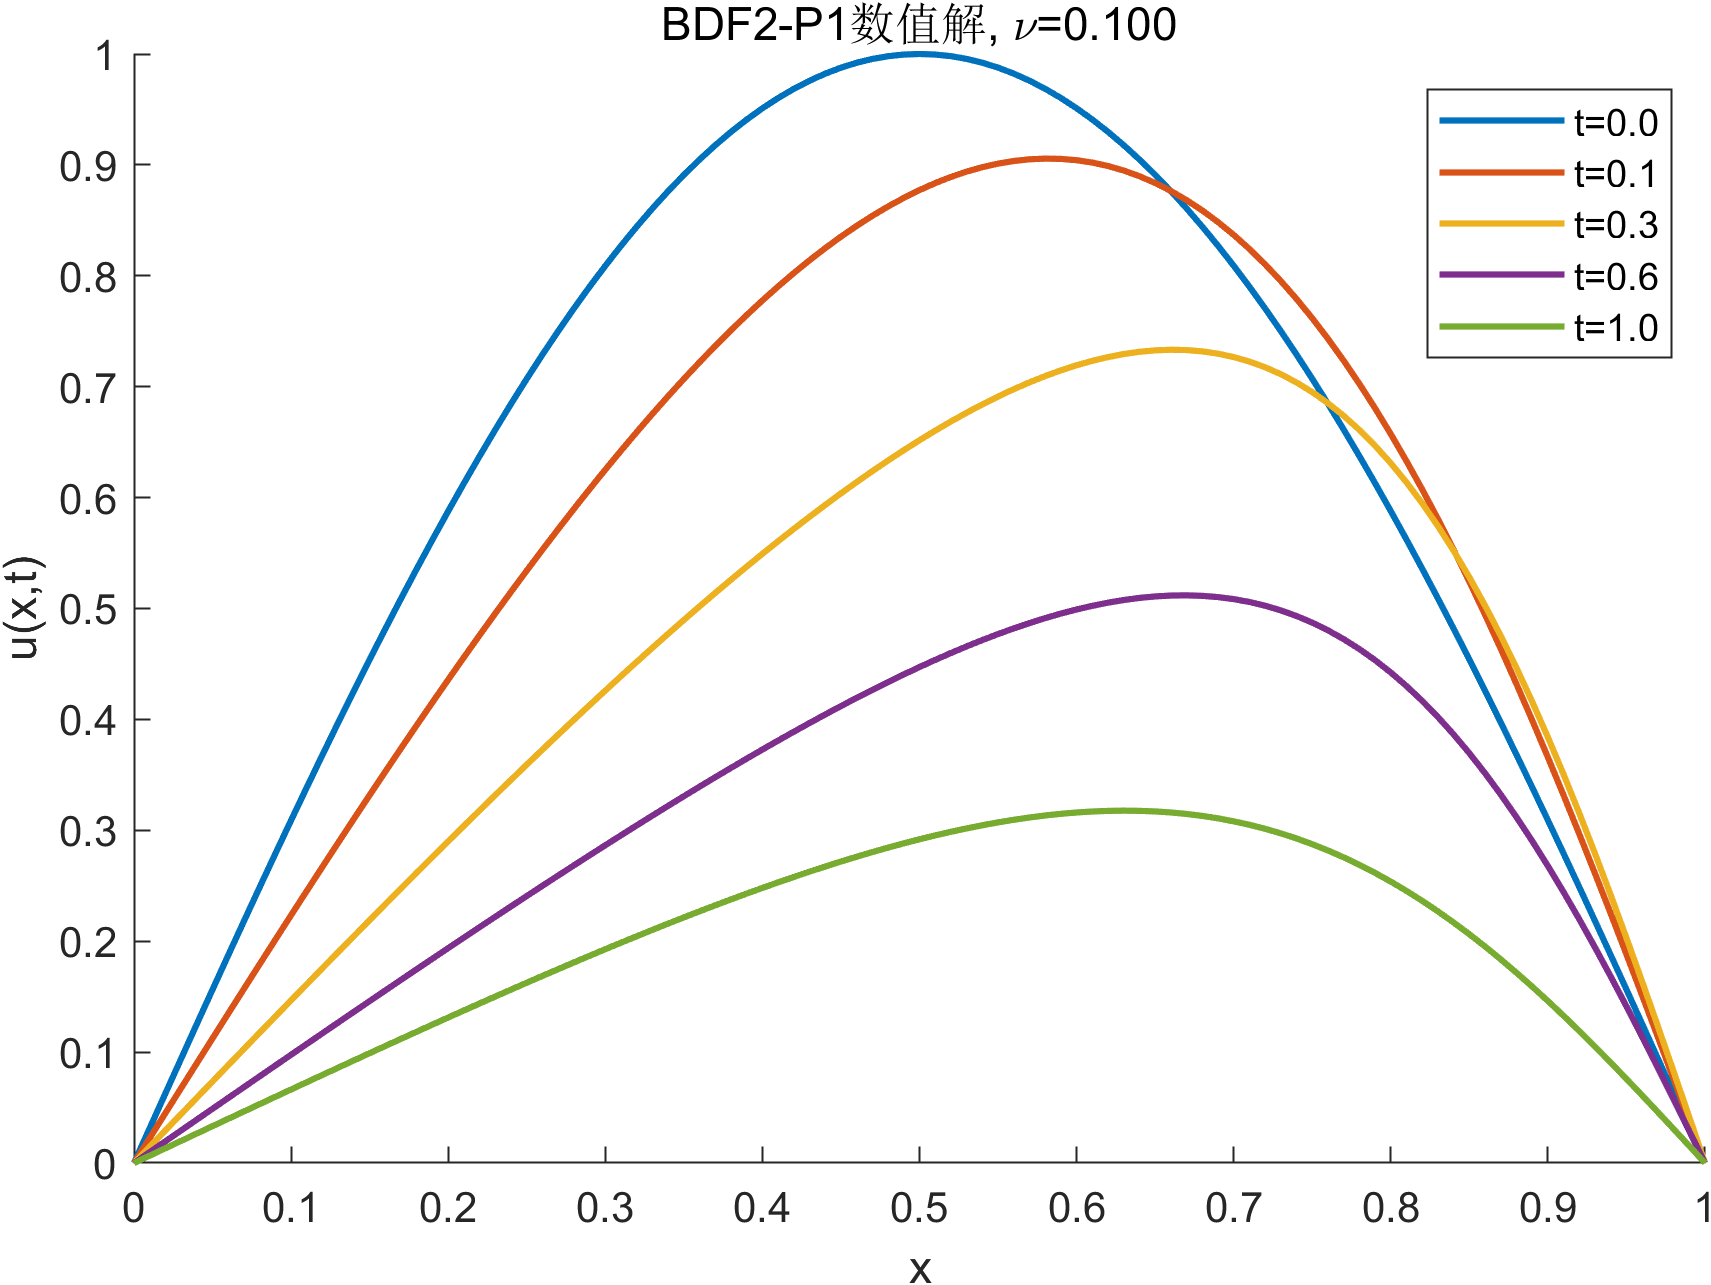
\includegraphics[width=0.5\linewidth]{nonlinear.png}
	\caption{BDF2-P1有限元数值解（$t=0,0.1,0.3,0.6,1.0$）}
	\label{fig:nonlinear_solution}
\end{figure}
\begin{table}[htbp]
	\centering
	\zihao{5}\songti
	\caption{BDF2-P1有限元方法在$t=0.1$时刻的数值解与解析解对比（算例4，$h=0.01$）}
	\label{tab:compare}
	\begin{tabular}{cccc}
		\toprule
		$x$ & 数值解 & 参考解析解 & $|u_h-u|$ \\
		\midrule
		0.1  & 0.22347 & 0.22345 & $2.0\times 10^{-5}$\\
		0.2  & 0.43584 & 0.43580 & $4.0\times 10^{-5}$\\
		0.3 & 0.62517 & 0.62512 & $5.0\times 10^{-5}$\\
		0.4 & 0.77776 & 0.77772  & $4.0\times 10^{-5}$\\
		0.5 & 0.87729 & 0.87728  & $1.0\times 10^{-5}$\\
		\bottomrule
	\end{tabular}
\end{table}
从图\ref{fig:nonlinear_solution}可以看出，利用BDF2-P1方法求解非线性问题\eqref{eq:nonlinear}进行数值求解，可获得在不同时刻（$t=0,0.1,0.3,0.6,1.0$）的数值解结果，图中可以清晰观察到问题\eqref{eq:nonlinear}的典型演化规律：初始时刻解为标准正弦分布，满足齐次Dirichlet边界条件；接着随着时间推进，非线性对流项推动波形峰值逐渐右移，而粘性扩散项则持续耗散能量，导致波形幅值不断衰减、整体逐渐展宽，最终随时间趋于零，完全符合抛物型方程的耗散特性。数值结果充分验证了BDF2-P1方法的有效性，即所有时刻的数值解均严格满足边界条件，无伪振荡与发散现象，体现了BDF2格式的无条件稳定性；P1线性有限元在$h=0.01$的网格下精准捕捉了波形的演化细节，无数值弥散，验证了该数值方法对非线性方程的求解可靠性。同时，从表格\ref {tab:compare}可以看出，本文的数值方法能够准确逼近真解，计算效果良好，同样验证了该方法的有效性与可靠性。
%\begin{remark}[复杂几何的网格生成]
%本文采用的三角形网格剖分技术同样适用于带有曲线边界或多连通区域的复杂几何。例如，对于带孔洞的区域$\Omega = (0,1)^2 \setminus \overline{B_{0.1}(0.5,0.5)}$，只需在FreeFEM++中定义内外边界即可自动生成非结构网格（如图\ref{fig:complete_mesh}所示），无需对数值格式做任何修改，这表明l本文方法具有良好的几何适应性。
%\begin{figure}[H]
%	\centering
%	\includegraphics[width=0.5\linewidth]{complete_mesh.eps}
%	\caption{复杂区域网格剖分示例}
%	\label{fig:complete_mesh}
%\end{figure}
%\end{remark}
\subsection{本章小结}
%本章构造了具有精确解的一维区域和二维规则区域上的热传导方程，对第三章的理论分析结果进行系统验证，并进一步将本文方法应用于非线性抛物型偏微分方程的数值求解。首先，针对一维热传导问题，实现了BDF2-P1有限元格式，通过引入向后欧拉法作为启动格式，解决了BDF2多步格式的初值依赖问题；并利用编程软件实现算法，其数值结果表明，所得到的数值解与解析解高度吻合，三维演化曲面的对比更是进一步直观地验证了方法的有效性。在收敛性分析方面，通过空间收敛性测试和时间收敛性测试，验证了其理论分析的正确性。同时，选取另一类初值问题进行数值验证，同样获得了理想的数值解形态，展示了该方法对不同问题的适应性。其次，本章的第二节将数值方法推广至二维热传导方程，本章借助FreeFEM++软件，使用三角形剖分，对具有解析解的算例进行了数值实验。最后，选取具有解析解非线性抛物型偏微分方程进行数值实验，探究其数值方法对非线性方程的有效性。综上，本章的数值实验不仅验证了全离散格式的理论收敛阶与稳定性，也展示了其在数值计算中的可靠性与适用性，为低维热传导问题的数值求解提供了有效的算法实现与实证支持。
本章构造了具有解析解的一维、二维规则区域热传导方程及非线性抛物型偏微分方程算例，验证第三章理论分析结果和本文数值方法的有效性。一维问题中，实现BDF2-P1有限元格式，以向后欧拉法解决初值依赖问题，数值结果与解析解高度吻合，收敛性测试验证了理论正确性，且该方法对不同初值问题具有适应性。二维问题借助FreeFem++软件和采用三角形剖分完成数值实验；非线性算例则验证了该数值方法对非线性方程的有效性。综上，本章的数值算例验证了全离散BDF2-P1格式的收敛阶与稳定性，证明其可靠性与适用性，为低维热传导问题求解提供了算法与实证支持。
\clearpage
\section{总结与展望}
本文介绍了利用有限元方法求解带齐次Dirichlet边界条件热传导方程的基本原理和方法，并构造了合适的数值算例，验证了其数值方法的有效性。本章将对全文做一个总结，并展望利用有限元方法数值求解偏微分方程的发展趋势。
\subsection{总结}
%本文围绕有限元方法数值求解热传导方程展开研究，系统阐述了如何将有限元方法与二阶向后差分格式相结合，构造热传导问题模型的半离散格式和全离散格式，通过理论分析、算法设计和数值实验，验证了该方法对求解热传导方程中的有效性和可靠性。
本文围绕有限元方法数值求解热传导方程展开研究。首先，在空间方向上采用分片线性有限元方法对热传导方程进行离散，将无穷维问题转化为有限维问题，并详细构造了基于节点基函数的有限元空间$V_h \subset H_0^1(\Omega)$；其次，在时间方向上引入二阶向后差分格式（BDF2），分别构造了空间半离散格式和全离散BDF2-P1格式，对半离散格式进行稳定性分析和误差估计；同时对于全离散BDF2-P1格式给出了严格的误差分析，证明了其在$L^2$范数意义下具有$O(h^2 + \tau^2)$的收敛阶，其中$h$为空间网格尺寸，$\tau$为时间步长；通过理论分析、算法设计以及一系列数值实验，验证了所提方法对求解热传导方程的有效性和可靠性；实验结果表明，BDF2-P1格式具有良好的数值稳定性，能够有效抑制非物理振荡。总的来说，利用有限元方法和二阶向后差分格式相结合的方法是一种可靠的数值方法，能够有效的求解热传导方程。
\subsection{展望}
有限元方法是一种重要的数值方法，在工程技术、科学计算等众多领域中占据重要地位，具有极为广泛的应用场景。在热方程求解领域，该方法的未来发展与优化改进，主要集中体现在以下三个核心层面：
在方法精度层面，可通过引入更高阶有限元空间与高阶时间离散格式，研发具备更高收敛阶的数值算法，进一步降低求解误差，提升热方程数值解的精准度，满足复杂热传导问题对计算精度的严苛要求；在模型推广层面，本文已将该数值方法成功应用于简单非线性热方程的求解，有效验证了有限元方法在非线性场景下的适用性与可靠性，未来可进一步拓展至更复杂的非线性体系，推动其在非线性热传导问题中的深度应用；在计算效率层面，可结合自适应网格加密技术、区域分解并行算法、深度学习代理模型等手段，大幅提升大规模、多尺度热传导问题的求解效率，破解传统有限元方法在处理复杂工程问题时的效率瓶颈，推动其在实际工程仿真中的规模化应用。未来，有限元方法将更加注重与其他数值方法的交叉融合，充分发挥各类方法的独特优势，着力攻克多物理场综合作用、复杂几何结构、高维热传导等核心技术难题，持续拓展其在科学计算与工程应用中的适用范围，进一步提升其实际应用价值。

\bibliographystyle{unsrtnat}   % 需要加载 natbib 宏包
%\bibliographystyle{unsrt}
\bibliography{examplebib} %参考文献

\thanks %致谢
2022年9月金秋，我怀揣着对大学生活的向往踏入校门。敲下“致谢”二字，这篇论文终成定稿，我的大学生涯也至此画上圆满的句点；四年光阴倏然而逝，往事历历如昨，方知往者不谏，来者犹可追。

落笔论文，幸得良师指导。刘鸿雁老师温柔细心，从论文选题、框架构思到反复修改直至定稿，始终耐心指引、悉心点拨，伴我一步步拨开迷雾、厘清思路，终至论文定稿。同时，我要感谢所有授课老师悉心教诲、倾囊相授，使我渐窥学术门径，受益终身。我将永远铭记学校的培育之恩、老师的教诲之情与同窗的相伴之谊，在人生路上脚踏实地、勇毅前行。

走到此刻，感谢所有成全与守护。最感恩这一路走来在身边陪伴的父母，始终无条件理解、支持与包容，做我最坚实的后盾，让我心无旁骛、勇敢奔赴，看见更辽阔的世界。感谢我的兄长，在我迷茫时给予坚定支持，在我困顿时提供情绪慰藉，让我得以坚守本心，追寻本真的自己。感谢一路相伴的朋友，于求学途中彼此鼓励、温暖同行，为成长岁月增添诸多光亮与欢喜。纵不擅言辞，然这份真挚谢意，想直白说与每一位帮助、陪伴我的人听。

求学之路道阻且长，眼泪与坚持皆为成长印记。感谢那个步履缓慢却从未轻言放弃的自己，一个本易半途而废的人，却在求知途中坚守至今。愿这份笨拙却坚定的执着，能伴我奔赴更远的山海；愿我们永远怀揣少年赤诚与明朗，不忘初心，砥砺前行。

谨以此文，致谢所有相遇与陪伴。祝诸位四时如意，万事遂心。


\appendix %附录
\begin{algorithm}
	\caption{BDF2-P1格式数值求解一维情形}
	\label{alg:BDF2-P1}
	\KwData{空间单元数 $N_x$，时间步数 $N_t$，终时 $T$，源项 $f(x)$}
	\KwResult{数值解 $\mathbf{u}^m\ (m=0,\dots,N_t)$}
	\BlankLine
	\textbf{Step 1: 网格与参数}\;
	$h \gets 1/N_x$, $\tau \gets T/N_t$\;
	生成节点 $\{x_j\}_{j=1}^{N_x+1}$ 与单元连接\;
	
	\BlankLine
	\textbf{Step 2: 组装矩阵}\;
	\ForEach{单元 $e=1,\dots,N_x$}{
		计算 $M^e, A^e$ (单元质量、刚度矩阵)\;
		组装至全局 $M, A$\;
		计算单元载荷 $\mathbf{F}^e$ (高斯积分) 并累加至 $\mathbf{F}$\;
	}
	
	\BlankLine
	\textbf{Step 3: 处理边界}\;
	边界节点 $\text{bdry}=\{1,N_x+1\}$, 自由节点 $\text{free}=\{2,\dots,N_x\}$\;
	提取子矩阵: $M_f, A_f, \mathbf{F}_f$\;
	
	\BlankLine
	\textbf{Step 4: 时间离散 (BDF2)}\;
	BDF2格式: $\left(\dfrac{3}{2\tau}M_f + A_f\right)\mathbf{u}_f^m = \dfrac{M_f}{2\tau}(4\mathbf{u}_f^{m-1} - \mathbf{u}_f^{m-2}) + \mathbf{F}_f$\;
	
	\BlankLine
	\textbf{Step 5: 时间步进}\;
	$\mathbf{u}_f^0 \gets \mathbf{0}$\;
	$\mathbf{u}_f^1 \gets \text{Solve}\big((\frac{1}{\tau}M_f + A_f), \frac{1}{\tau}M_f\mathbf{u}_f^0 + \mathbf{F}_f\big)$ \tcp*{BDF1启动}
	\For{$m=2$ \KwTo $M$}{
		$\mathbf{u}_f^m \gets \text{Solve}\big((\frac{3}{2\tau}M_f + A_f), \frac{M_f}{2\tau}(4\mathbf{u}_f^{m-1} - \mathbf{u}_f^{m-2}) + \mathbf{F}_f\big)$\;
	}
	
	\BlankLine
	\textbf{Step 6: 重构与输出}\;
	\For{$m=0$ \KwTo $N_t$}{
		$\mathbf{u}^m[\text{free}] \gets \mathbf{u}_f^m$, $\mathbf{u}^m[\text{bdry}] \gets 0$\;
	}
	\KwRet{$\{\mathbf{u}^m\}_{m=0}^{N_t}$}\;
\end{algorithm}
\clearpage %每章/节之间要求分页
\begin{algorithm}
	\caption{BDF2-P1格式数值求解二维情形}
	\label{alg:BDF2_optimized}
	\KwData{扩散系数 $\alpha$，最终时间 $T$，空间剖分数 $N_x$，时间步数 $N_t$，源项 $f(x,y,t)$}
	\KwResult{数值解 $\{u^n\}_{n=0}^{N_t} \subset V_h$ 及各时间层误差}
	\BlankLine
	\textbf{Step 1: 网格与参数}\;
	$h \gets 1/N_x$, $\tau \gets T/N_t$\;
	生成区域 $\Omega = (0,1)^2$ 的均匀三角形剖分 $\mathcal{T}_h$，网格尺寸 $h = 1/N_x$\;
	
	\BlankLine
	\textbf{Step 2: 定义有限元空间}\;
	定义 $P_1$ 有限元空间：
	\[
	V_h = \left\{ v_h \in C^0(\overline{\Omega}): \left. v_h \right|_K \in \mathbb{P}_1,\ \forall K \in \mathcal{T}_h,\ \left. v_h \right|_{\partial\Omega}=0 \right\}
	\]
	
	\BlankLine
	\textbf{Step 3: 初始化}\;
	$u^0 \gets 0$, $u^{-1} \gets 0$, 并令 $n = 1$\;
	
	\BlankLine
	\textbf{Step 4: 时间离散格式}\;
	BDF1格式（起步）：
	\[
	\frac{1}{\tau}(u^n, v) + \alpha(\nabla u^n, \nabla v) = \frac{1}{\tau}(u^{n-1}, v) + (f^n, v), \quad \forall v \in V_h
	\]
	BDF2格式：
	\[
	\frac{3}{2\tau}(u^n, v) + \alpha(\nabla u^n, \nabla v) = \frac{1}{2\tau}(4u^{n-1} - u^{n-2}, v) + (f^n, v), \quad \forall v \in V_h
	\]
	
	\BlankLine
	\textbf{Step 5: 时间步进}\;
	\For{$n=1$ \KwTo $N_t$}{
		$t \gets n\tau$\;
		更新源项 $f^n = f(x,y,t)$\;
		
		\eIf{$n = 1$}{
			$u^n \gets \text{Solve}\big(\text{BDF1格式}, \frac{1}{\tau}u^{n-1} + f^n\big)$ \tcp*{BDF1启动}
		}{
			$u^n \gets \text{Solve}\big(\text{BDF2格式}, \frac{1}{2\tau}(4u^{n-1} - u^{n-2}) + f^n\big)$\;
		}
		
		\If{$n \bmod 20 = 0$ \textbf{or} $n = N_t$}{
			计算精确解 $u_{\text{ex}}^n = \dfrac{1}{2\pi^2-1}(e^{-t} - e^{-2\pi^2 t})\sin(\pi x)\sin(\pi y)$\;
			计算 $L^2$ 误差 $\|u^n - u_{\text{ex}}^n\|_{L^2(\Omega)}$ 并输出\;
		}
		
		更新历史数据：$u^{n-2} \leftarrow u^{n-1}$，$u^{n-1} \leftarrow u^n$\;
	}
	
	\BlankLine
	\textbf{Step 6: 后处理}\;
	计算最终时刻全局 $L^2$ 误差 $\|u^{N_t} - u_{\text{ex}}^T\|_{L^2(\Omega)}$\;
	绘制数值解图像 $\text{plot}(u^{N_t})$\;
	\KwRet{$\{u^n\}_{n=0}^{N_t}$ 及误差结果}\;
\end{algorithm}
\clearpage
\begin{algorithm}
	\caption{BDF2-P1 格式求解非线性方程}
	\label{alg:BDF2-P1-nonlinear-simple}
	\KwData{空间剖分数 $N$，时间步长 $\Delta t$（最终调整），终时 $T$，粘性系数 $\nu$，初始条件 $u_0(x)$，牛顿容差 $tol$，最大迭代次数 $maxIter$}
	\KwResult{数值解 $\{u_h^n\}_{n=0}^{N_t}$（全节点值）}
	\BlankLine
	\textbf{Step 1: 空间离散}\;
	生成均匀网格 $x_j = jh,\; j=0,\dots,N$，$h=1/N$\;
	定义自由度映射（内部节点为自由度，边界节点固定为0）\;
	组装全局质量矩阵 $M$ 与刚度矩阵 $A$（标准线性有限元）\;
	\BlankLine
	\textbf{Step 2: 初始条件}\;
	$\mathbf{u}^0 \gets u_0(x)$ 在自由节点上的值\;
	\BlankLine
	\textbf{Step 3: BDF1 启动步（向后欧拉）}\;
	求解 $\left(\frac{1}{\Delta t}M + \nu A\right)\mathbf{u}^1 + \mathbf{N}(\mathbf{u}^1) = \frac{1}{\Delta t}M\mathbf{u}^0$\;
	（牛顿迭代，初值 $\mathbf{u}^1_0 = \mathbf{u}^0$）\;
	\BlankLine
	\textbf{Step 4: BDF2 主循环}\;
	\For{$n = 2$ to $N_t$（$N_t = T/\Delta t$）}{
		求解 $\left(\frac{3}{2\Delta t}M + \nu A\right)\mathbf{u}^n + \mathbf{N}(\mathbf{u}^n) = \frac{2}{\Delta t}M\mathbf{u}^{n-1} - \frac{1}{2\Delta t}M\mathbf{u}^{n-2}$\;
		牛顿迭代初值：$\mathbf{u}^n_0 = 2\mathbf{u}^{n-1} - \mathbf{u}^{n-2}$（外推）\;
	}
	\BlankLine
	\textbf{Step 5: 非线性项处理}\;
	在每个单元上，由自由节点值 $u_1, u_2$ 计算对流贡献及雅可比矩阵，组装到全局残差 $\mathbf{N}$ 和全局雅可比 $\mathbf{J}_N$\;
	\BlankLine
	\textbf{Step 6: 牛顿迭代}\;
	\Repeat{$\|\mathbf{F}\|_\infty < tol$ 或 达到 $maxIter$}{
		计算总残差 $\mathbf{F} = \big(\alpha M + \nu A\big)\mathbf{u} + \mathbf{N}(\mathbf{u}) - \mathbf{rhs}$\;
		计算总雅可比 $\mathbf{J} = \alpha M + \nu A + \mathbf{J}_N(\mathbf{u})$\;
		求解 $\mathbf{J}\,\boldsymbol{\delta} = -\mathbf{F}$\;
		更新 $\mathbf{u} \gets \mathbf{u} + \boldsymbol{\delta}$\;
	}
	\BlankLine
	\textbf{Step 7: 输出}\;
	边界节点补零得到全节点解 $\{U^n\}$\;
	\KwRet{$\{U^n\}$}
\end{algorithm}
%\section*{常用不等式}
%
%
%\section*{代码}
%\begin{lstlisting}[
%	language=MATLAB,
%	caption={一维线性有限元基函数可视化MATLAB代码},
%	label={code:matlab-fem},
%	frame=single,
%	numbers=left,
%	basicstyle=\ttfamily\small,
%	keywordstyle=\color{blue}\bfseries,
%	commentstyle=\color{gray}\itshape,
%	breaklines=true,
%	showstringspaces=false,
%	numbersep=5pt
%	]
%   clear;
%   L = 1;
%   Ne = 5;
%   h = L/Ne;
%   x = 0:h:L;
%   figure('Position', [100, 100, 600, 400]);
%   hold on;
%   for i = 2:Ne
%   plot([x(i-1), x(i), x(i+1)], [0, 1, 0], 'b-', 'LineWidth', 2);
%   text(x(i), 1.05, sprintf('φ_%d', i), 'HorizontalAlignment', 'center');
%   end
%   plot(x, zeros(size(x)), 'ko', 'MarkerFaceColor', 'k');
%   for i = 1:length(x)
%   text(x(i), -0.05, sprintf('x_%d', i), 'HorizontalAlignment', 'center');
%   end
%   grid on;
%   xlim([-0.05, L+0.05]);
%   ylim([-0.1, 1.2]);
%   xlabel('x');
%   ylabel('φ_i(x)');
%   title(sprintf('一维线性有限元基函数 (Ne=%d)', Ne));
%   hold off;
%\end{lstlisting}
%
%\begin{lstlisting}[
%	language=MATLAB,
%	caption={BDF2-P1有限元求解一维热传导方程主函数MATLAB代码},
%	label={code:matlab-main},
%	frame=single,
%	numbers=left,
%	basicstyle=\ttfamily\small,
%	keywordstyle=\color{blue}\bfseries,
%	commentstyle=\color{gray}\itshape,
%	breaklines=true,
%	showstringspaces=false,
%	numbersep=5pt
%	]
%	clear;
%	alpha=1;
%	A=2;
%	L=1;
%	T_final=1;
%	%离散参数
%	Nx=50;
%	h=L/Nx;
%	Nt=100;
%	tau=T_final/Nt;
%	verbose=true;     %显示详细信息
%	plot_results=true;   %绘制结果
%	[solution,errors]=solve_BDF2_P1(alpha,A,L,T_final,Nx,Nt);
%	if verbose
%	fprintf('==========================================\n');
%	fprintf('数值求解结果\n');
%	fprintf('==========================================\n');
%	fprintf('扩散系数:%.2f\n',alpha);
%	fprintf('源项振幅:%.2f\n',A);
%	fprintf('区间长度:%.2f\n',L);
%	fprintf('终时:%.2f\n',T_final);
%	fprintf('空间单元数:%d,节点数:%d\n',Nx,solution.Nn);
%	fprintf('时间步数:%d\n',Nt);
%	fprintf('空间步长:h=%.4f\n',h);
%	fprintf('时间步长:τ=%.4f\n',tau);
%	fprintf('------------------------------------------\n');
%	fprintf('L2误差:%.6e\n',errors.L2);
%	fprintf('最大误差:%.6e\n',errors.max);
%	fprintf('==========================================\n');
%	end
%	if plot_results&&isfield(solution,'x_nodes')&&isfield(solution,'u_numerical')
%	figure('Position',[100,100,1200,500]);
%	plot(solution.x_nodes,solution.u_exact,'b-','LineWidth',2.5);
%	hold on;
%	plot(solution.x_nodes,solution.u_numerical,'r--','LineWidth',1.8);
%	xlabel('$x$','Interpreter','latex','FontSize',13);
%	ylabel('$u(x,t)$','Interpreter','latex','FontSize',13);
%	title(sprintf('BDF2-P1有限元数值解(Nx=%d,Nt=%d)',Nx,Nt),...
%	'FontSize',14,'FontWeight','bold');
%	grid on;
%	xticks(0:0.2:1);
%	yticks(0:0.05:0.25);
%	xlim([0,1]);
%	ylim([0,0.25]);
%	legend({'解析解','数值解(BDF2-P1)'},...
%	'FontSize',11,'Location','northwest','Box','off');
%	end
%\end{lstlisting}
%
%\begin{lstlisting}[
%	language=MATLAB,
%	caption={BDF2-P1有限元求解一维热传导方程的关键函数MATLAB代码},
%	label={code:matlab-solve-BDF2-P1},
%	frame=single,
%	numbers=left,
%	basicstyle=\ttfamily\small,
%	keywordstyle=\color{blue}\bfseries,
%	commentstyle=\color{gray}\itshape,
%	breaklines=true,
%	showstringspaces=false,
%	numbersep=5pt
%	]
%	function [solution,errors]=solve_BDF2_P1(alpha,A,L,T_final,Nx,Nt)
%	h=L/Nx;
%	tau=T_final/Nt;
%	Nn=Nx+1;
%	[x_nodes,elements]=generate_mesh(L,Nx);
%	[M,A_mat,F,free_nodes]=assemble_matrix(x_nodes,elements,alpha,A,h);
%	[U_all,time]=time_marching_BDF2(M,A_mat,F,free_nodes,Nn,Nt,tau);
%	u_exact=compute_exact_solution(x_nodes,T_final,A,alpha);
%	u_numerical=U_all(:,end);
%	errors=compute_errors(u_numerical,u_exact,h);
%	solution.x_nodes=x_nodes;
%	solution.elements=elements;
%	solution.U_all=U_all;
%	solution.Nn=Nn;
%	solution.time=time;
%	solution.u_exact=u_exact;
%	solution.u_numerical=u_numerical;
%	solution.h=h;
%	solution.tau=tau;
%	end
%\end{lstlisting}
%
%\begin{lstlisting}[
%	language=C++,
%	caption={二维非齐次热方程的FreeFEM++求解代码},
%	label={code:heat2d-bdf2},
%	frame=single,
%	numbers=left,
%	basicstyle=\ttfamily\small,
%	keywordstyle=\color{blue}\bfseries,
%	commentstyle=\color{gray}\itshape,
%	breaklines=true,
%	showstringspaces=false,
%	numbersep=5pt
%	]
%	real alpha=1.0;      
%	real T=1.0;          
%	real L=1.0;          
%	func real uexact(real xx,real yy,real tt) {
%		return (1.0/(1.0+2.0*pi*pi*alpha))*
%		(exp(-tt)-exp(-2.0*pi*pi*alpha*tt))*sin(pi*xx)*sin(pi*yy);
%	}
%	func real source(real xx,real yy,real tt) {
%		return exp(-tt)*sin(pi*xx)*sin(pi*yy);
%	}
%	int Nx=50;           
%	real h=L/Nx;         
%	int Nsteps=100;      
%	real tau=T/Nsteps;       
%	cout << "=====================================================" << endl;
%	cout << "2D nonhomogeneous heat equation numerical solution" << endl;
%	cout << "Parameters: alpha = " << alpha << ", T = " << T << ", Nx = " << Nx << endl;
%	cout << "Space step h = " << h << ", Time step tau = " << tau << endl;
%	cout << "=====================================================" << endl;
%	mesh Th=square(Nx,Nx);
%	fespace Vh(Th,P1);
%	Vh u, v;               
%	Vh uold, uold2;        
%	Vh f, uex;             
%	u=0;
%	uold=0;
%	uold2=0;
%	real t=tau;
%	f=source(x,y,t);
%	problem HeatInit(u,v) = 
%	int2d(Th)(u*v/tau+alpha*(dx(u)*dx(v)+dy(u)*dy(v)))
%	-int2d(Th)(uold*v/tau+f*v)
%	+on(1,2,3,4, u=0);  
%	HeatInit;
%	uold2=uold;  
%	uold=u;      
%	uex=uexact(x,y,t);
%	real L2error=sqrt(int2d(Th)((u-uex)^2));
%	cout << "t = " << t << " (n=1): L2error = " << L2error << endl;
%	problem HeatBDF2(u,v) = 
%	int2d(Th)((3.0*u*v)/(2.0*tau)+alpha*(dx(u)*dx(v)+dy(u)*dy(v)))
%	- int2d(Th)((4.0*uold-uold2)*v/(2.0*tau)+f*v )
%	+ on(1,2,3,4, u=0);
%	for (int n=2;n<= Nsteps;n++) {
%		t=n*tau;
%		f=source(x,y,t);  
%		HeatBDF2;
%		if (n%20==0 || n==Nsteps) {
%			uex=uexact(x,y,t);
%			L2error=sqrt(int2d(Th)((u-uex)^2));
%			cout << "t = " << t << " (n=" << n << "): L2error= " << L2error << endl;
%		}
%		uold2=uold;  
%		uold=u;      
%	}
%	cout << "=====================================================" << endl;
%	cout << "Computation finished | Final time t = " << T << endl;
%	uex=uexact(x, y, T);
%	L2error=sqrt(int2d(Th)((u-uex)^2));
%	cout << "Global L2 error = " << L2error << endl;
%	cout << "=====================================================" << endl;
%	plot(u, fill=true, value=true, wait=false, cmm="Numerical Solution u_h", ps="numerical_solution.eps");
%\end{lstlisting}
\end{document}